%\documentclass[a4paper]{article}
%\usepackage[top=1in, bottom=1.25in, left=1.25in, right=1.25in]{geometry}
%\usepackage{amsmath}
%\usepackage{multicol}
%\usepackage{graphicx}
%\usepackage{subfig}
%\usepackage{amssymb}
%%\RequirePackage{ltxcmds}[2010/12/07]
%%opening
%\title{Linear Filtering in Frequency-Domain}
%\author{ }
%\date{ }
%\begin{document}
%
%\maketitle
\clearpage
\section{Overlap-Save Method}
\begin{tcolorbox}	
	\begin{tabular}{p{2.75cm} p{0.2cm} p{10.5cm}} 	
		\textbf{Header File}   &:&overlap\_save\_*.h \\
		\textbf{Source File}   &:&overlap\_save\_*.cpp \\
		\textbf{Version}       &:& 20180201 (Romil Patel)
	\end{tabular}
\end{tcolorbox}
Overlap-save is an efficient way to evaluate the discrete convolution between a very long signal and a finite impulse response (FIR) filter. The overlap-save procedure cuts the signal into equal length segments with some overlap and then it performs convolution of each segment with the FIR filter.
%Linear filtering can be easily implemented in time-domain resorting to the use of finite impulse response (FIR) digital filters and convolution property as,
%\begin{equation}
%    y(n)= \sum\limits_{k=0}^{R-1} x(n-k)h\left(k\right),
%    \label{genFIR}
%\end{equation}
%where $x(n)$ is the input signal, $h(k)$ is the FIR filter coefficients, $R$ is the length of FIR filter coefficients and $y(n)$ represents the filtered output signal.
%Analysing this equation we can note that, for a block signal of length $R$, the required number of operations for the direct implementation of equation~\eqref{genFIR} evolves with $R^2$, $\mathcal{O}(R^2)$. This limitation imposed the emergence of algorithm, where the linear convolution is calculated faster than the directly implementing of \eqref{genFIR}.
%In this sense, it is used the computation of linear filtering in frequency domain resorting to the use of fast Fourier transform (FFT) and inverse fast Fourier transform (IFFT) algorithms as
%However, for long input sequence, the direct implementation of frequency domain filtering in real-time is limited by the limited memory of the digital processors.
%Hence, the filtering in frequency-domain is implemented by sectioning or block the input signal, such that the practical implementation  of FFT and IFFT is feasible. In order to implement the non-cyclic convolution with the finite-length of cyclic convolution that the FFT provides, overlap-save and overlap-add method are use, enabling that the complexity evolves in log scale $\mathcal{O}(N\log_2N)$. The general method is to split the input signal into manageable blocks, then apply the FFT to to perform the linear convolution and at the end recombine the output blocks such that it is avoided the wrap-around errors due to the circular convolution imposed by FFT.
The overlap-save method can be computed in the following steps:\\
\textbf{ Step 1 :} Determine the length $M$ of impulse response, $h(n)$.\\ \\ 
\textbf{ Step 2 :} Define the size of FFT and IFFT operation, $N$. The value of $N$ must greater than $M$ and it should in the form $N = 2^k$ for the efficient implementation.\\ \\
\textbf{ Step 3 :} Determine the length $L$ to section the input sequence $x(n)$, considering that $N=L+M-1$.\\ \\   
\textbf{ Step 4 :} Pad $L-1$ zeros at the end of the impulse response $h(n)$ to obtain the length $N$.\\ \\
\textbf{ Step 5 :} Make the segments of the input sequences of length $L$, $x_i(n)$, where index $i$ correspond to the $i^{th}$ block. Overlap $M-1$ samples of the previous block at the beginning of the segmented block to obtain a block of length $N$. In the first block, it is added $M-1$ null samples.\\ \\
\textbf{ Step 6 :} Compute the circular convolution of segmented input sequence $x_i(n)$ and $h(n)$ described as,
\begin{equation}
y_i(n)= x_i(n) \circledast h(n).
\label{genFIR}
\end{equation}
This is obtained in the following steps:\\
\textbf{1. } Compute the FFT of $x_i$ and $h$ both with length $N$.\\
\textbf{2. }Compute the multiplication of $X_i(f)$ and the transfer function $H(f)$.\\
\textbf{3. }Compute the IFFT of the multiplication result to obtain the time-domain block signal, $y_i$.\\ \\
\textbf{ Step 7 :} Discarded $M-1$ initial samples from the $y_i$, and save only the error-free $N-M-1$ samples in the output record.\\ \\
In the Figure~\ref{overlapSave} it is illustrated an example of overlap-save method.
\begin{figure}[h]
	\centering
	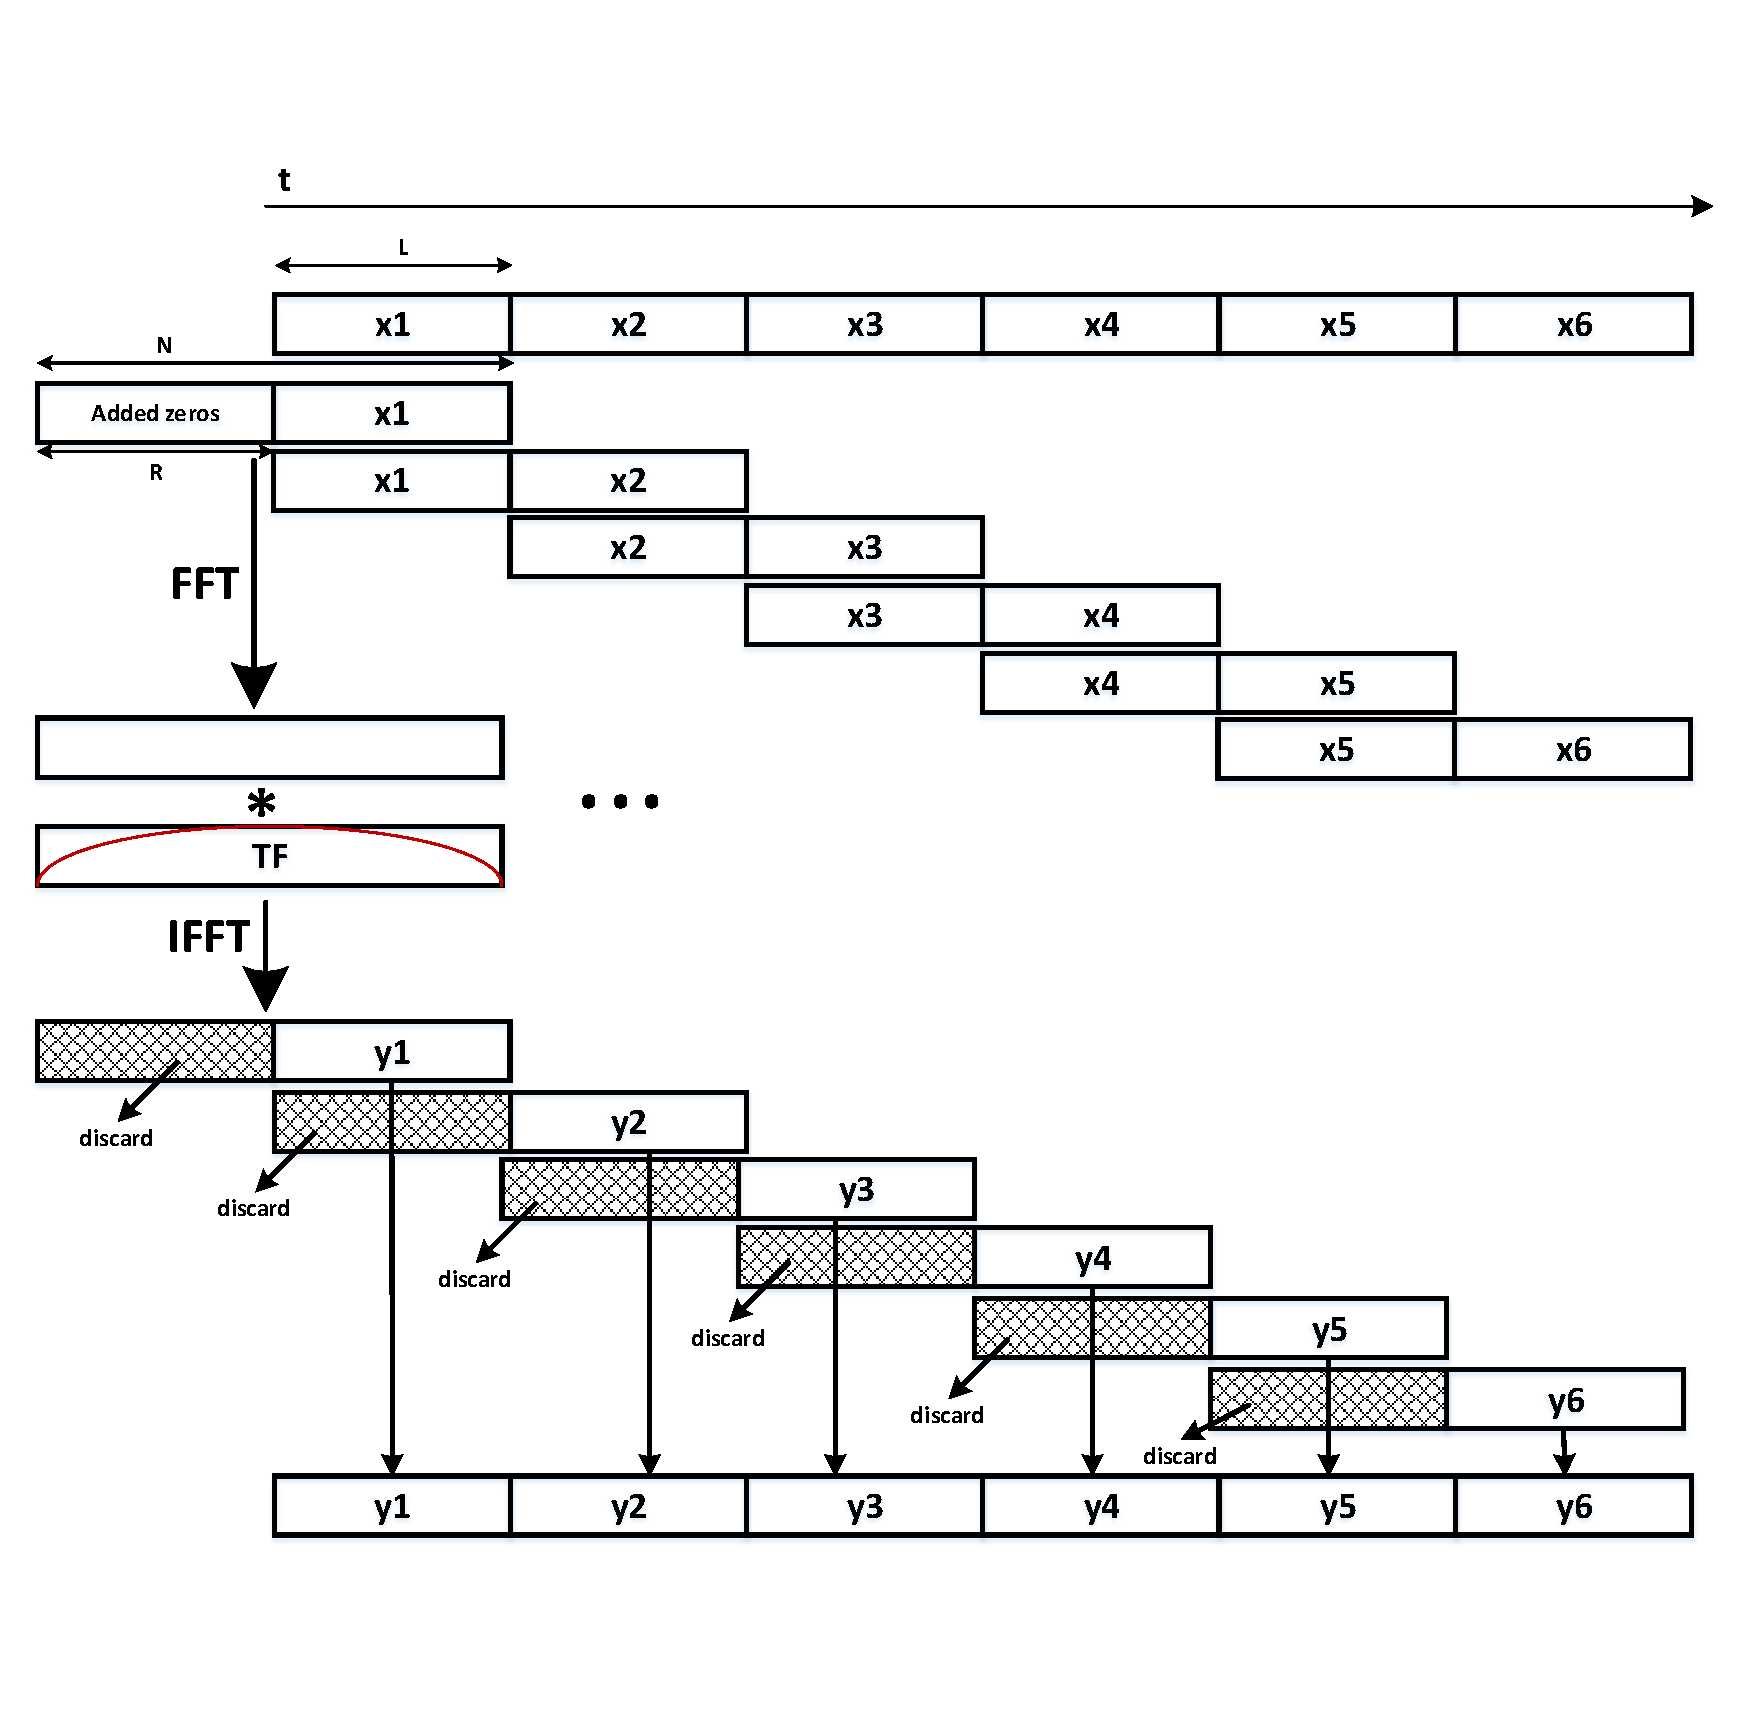
\includegraphics[width=12cm]{./algorithms/overlap_save/figures/overlap-savev2.pdf}
	\caption{Illustration of Overlap-save method.}
	\label{overlapSave}
\end{figure}

%\subsection*{Frequency response of filter}
%The frequency response of filter can be directly defined by using the frequency-domain formula, or it can be equivalently calculated from the FFT of impulse response of the filter. In this sense, we present an example of FIR filter (\textit{raised-cosine filter}) to illustrate these two cases.
%\begin{figure}[h]
%    \centering
%    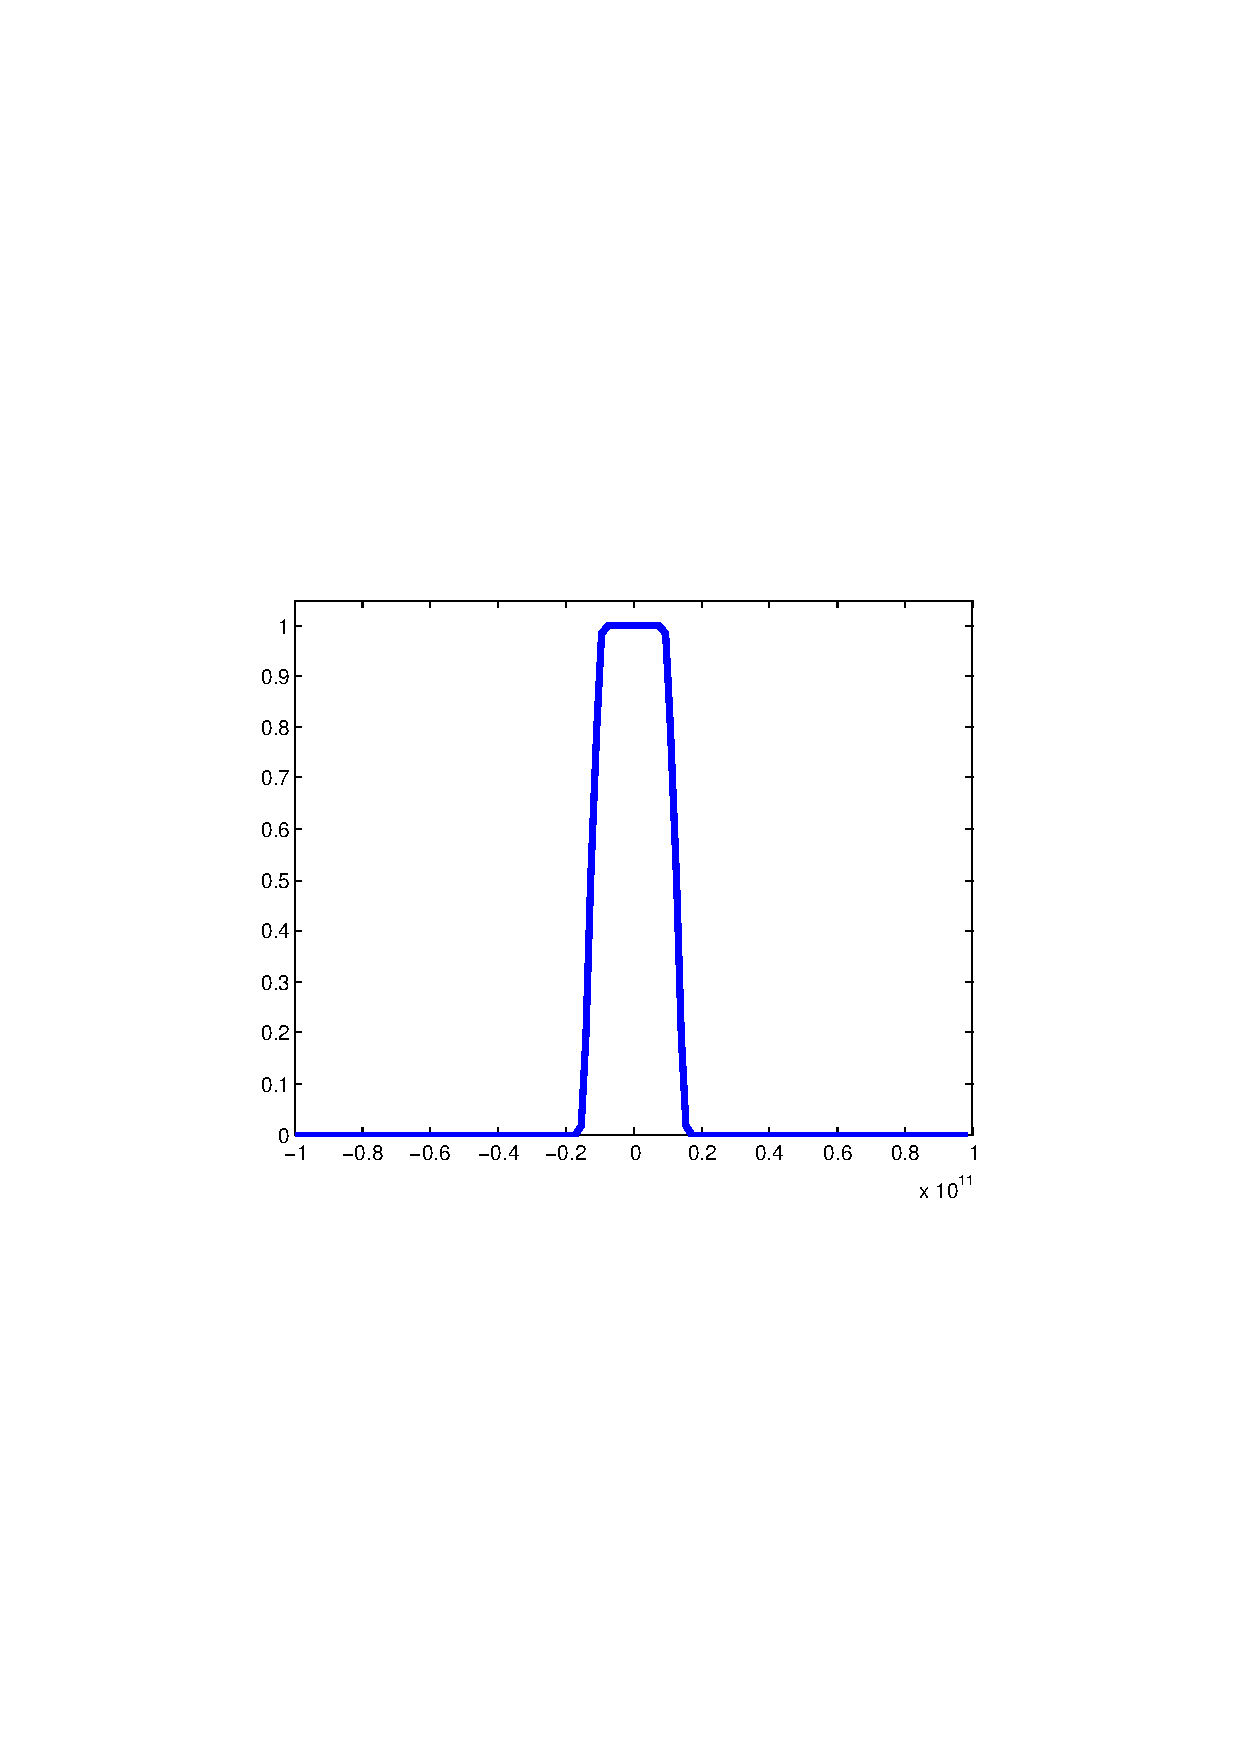
\includegraphics[width=6cm]{./algorithms/overlap_save/figures/rc-fd-filter-SpS8.pdf}
%    \caption{Frequency response of raised-cosine filter.}
%    \label{freq_rc}
%\end{figure}

%
%\subsubsection{Frequency-domain Formula}
%The frequency-domain description of raised-cosine filter can be given as,
%$$
%H(f) = \left\{
%    \begin{array}{ll}
%        1,       & \quad \left|f\right| \leq \frac{1-\beta}{2T} \\
%    \frac{1}{2}\left[ 1+\cos\left(\frac{\pi T}{\beta}\left[\left|f\right| - \frac{1-\beta}{2T}\right]\right)\right],  & \quad \frac{1-\beta}{2T} < \left|f\right| \leq \frac{1+\beta}{2T}\\
%    0, & \quad \text{otherwise}
%    \end{array}
%\right.
%$$
%where, $f$ is the frequency, $0 \leq \beta \leq 1$ corresponds to the roll-off factor and $T$ is the reciprocal of the symbol-rate.
%A plot of direct implementation of frequency response of raised-cosine filter is presented in Figure~\ref{freq_rc}, for a roll-off factor of 0.3.
%The frequency response, $H(f)$, calculated for $N$ frequency bins, which can be defined as,
%\begin{equation}
%    f= -\frac{fwindowTF}{2}:\frac{fwindowTF}{N}:\left(\frac{fwindowTF}{2}-\frac{fwindowTF}{N}\right),
%    \label{freq}
%\end{equation}
%where $fwindowTF$ is the sampling frequency. This, imposes that the length of $H(f)$ is $N$ as expected for the $N$-point FFT and the transfer function multiplication.
%\subsubsection{FFT of Impulse Response}
%Alternatively to the frequency-domain formula, we can obtain the frequency response of filter by calculating the FFT of its impulse response. In the case of raised-cosine filter, the impulse response is given as,
%
%\begin{equation}
%    h(t)= \frac{\sin(\pi t/T)}{\pi t/T}\frac{\cos(\pi t \beta/T)}{1-(2\beta t/T)^2},
%    \label{hn}
%\end{equation}
%where $t$ is the time. Figure~\ref{td_rc} shows a plot of impulse response of raised-cosine filter for a roll-off factor of 0.3.
%\begin{figure}[h!]
%    \centering
%    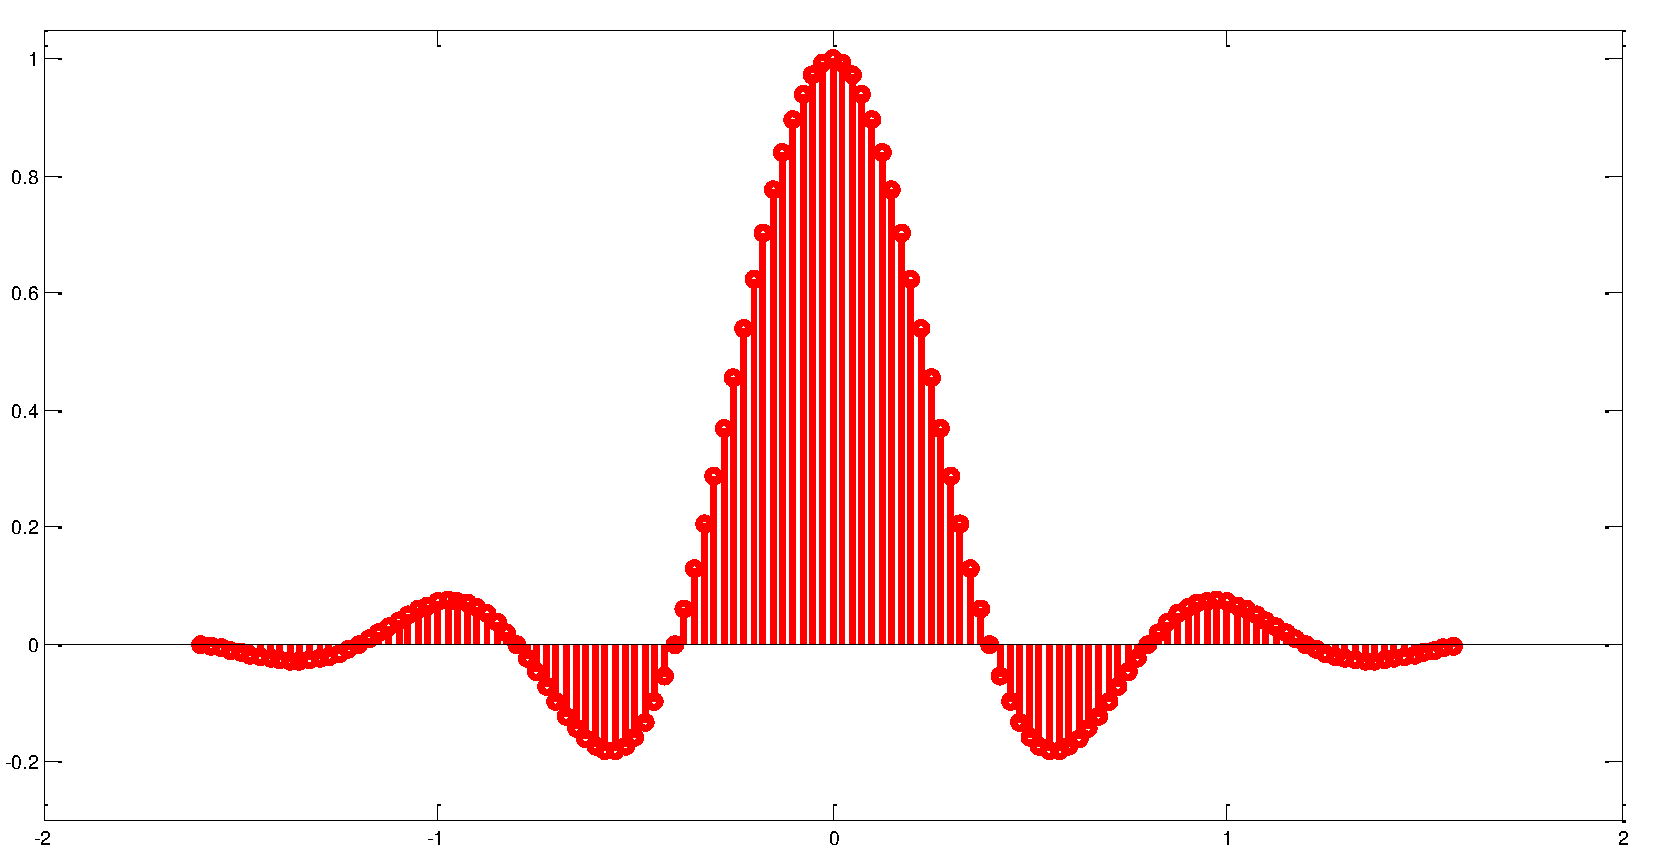
\includegraphics[width=8cm]{./algorithms/overlap_save/figures/rc-td-filter-stemv2.pdf}
%    \caption{Impulsee response of raised-cosine filter.}
%    \label{td_rc}
%\end{figure}
%Before calculating the FFT of the impulse response we must zero-pad the impulse response, which has the length $R$, to the length $N$. In this case $N$ is the FFT length, which is efficiently defined as power of 2. The zero-padding process can be performed by appending $L-1$ zeros at the end of impulse response, as shown in the Figure~\ref{zp-hn}.
%
%\begin{figure}[h]
%    \centering
%    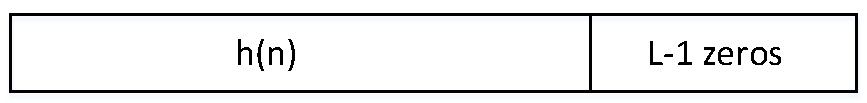
\includegraphics[width=6cm]{./algorithms/overlap_save/figures/zp-hn.pdf}
%    \caption{Zero-padding of impulse response $h(n)$.}
%    \label{zp-hn}
%\end{figure}

%
%In both cases, the frequency response of the filter will be limited to the frequency interval $fwindowTF$, [$-\frac{fwindowTF}{2}$, $\frac{fwindowTF}{2}$], and this range show us the $N$ frequency components obtained from FFT. The minimum frequency bin is $-\frac{fwindowTF}{2}$ and the maximum bin is $\frac{fwindowTF}{2}$, in which $fwindowTF$ corresponds to the sampling frequency. We can note that the spectral width of $H(f)$ is $fwindowTF$, which is the inverse of sampling period, $\mathop{dt}$. It is also important to note that, for a given sampling frequency, the frequency resolution, $\Delta f$, of $H(f)$ depends on the parameter $N$ and it increases with $N$, $\Delta f=\frac{fwindowTF}{N}$.


\tikzstyle{decision} = [diamond, draw, fill=white!20, 
text width=9em, text badly centered, node distance=3cm, inner sep=0pt]
\tikzstyle{block} = [rectangle, draw, fill=white!20,
text width=25em, text centered, rounded corners, minimum height=4em]
\tikzstyle{line} = [draw, -latex']
\tikzstyle{cloud} = [draw, ellipse,fill=white!20, node distance=3cm,
minimum height=3em]

\newpage
\subsection*{Function description}
Traditionally, overlap-save method performs the convolution (More precisely, circular convolution) between discrete time-domain signal $x(n)$ and the filter impulse response $h(n)$. Here the length of the signal $x(n)$ is greater than the length of the filter $h(n)$.
To perform convolution between the time domain signal $x(n)$ with the filter $h(n)$, include the header file overlap\_save\_*.h and then supply input argument to the function as follows,
 \begin{equation*}
 y(n) = overlapSave(x(n),h(n))
 \end{equation*}
Where, $x(n)$, $h(n)$ and $y(n)$ are of the C++ type vector< complex<double> > and the length of the signal $x(n)$ and filter  $h(n)$ could be arbitrary.\\
The one noticeable thing in the traditional way of implementation of overlap-save is that it cannot work with the real-time system. Therefore, to make it usable in the real-time environment, one more $overlapSave$ function with three input parameters was implemented and used along with the traditional overlap-save method. The structure of the new function is as follows,
 \begin{equation*}
y(n) =overlapSave(x_{m}(n), x_{m-1}(n), h(n))
\end{equation*}
Here, $x_{m}(n)$, $x_{m-1}(n)$ and $h(n)$ are of the C++ type vector< complex<double> > and the length of each of them are arbitrary. However, the combined length of $x_{m-1}(n)$ and $x_{m}(n)$ must be greater than the length of $h(n)$.
\subsection*{Linear and circular convolution}
In the circular convolution, if we determine the length of the singal $x(n)$ is $N_{1} = 8$ and length of the filter is  $h(n)$ is $N_{2} = 5$; then the length of the output signal is determined by $N = max(N_{1} , N_{2} )=8$. Next, the circular convolution can be performed after padding $0$ in the filter $h(n)$ to make it's length equals $N$. \\ \\
In the linear convolution, if we determine the length of the signal $x(n)$ is $N_{1} = 8$ and length of the filter is  $h(n)$ is $N_{2} = 5$; then the length of the output signal is determined by $N = N_{1}+N_{2}-1 = 12$. Next, the linear convolution using circular convolution can be performed after padding $0$ in the signal $x(n)$ filter $h(n)$ to make it's length equals $N$.

\subsection*{Flowchart of real-time overlap-save method}
\begin{figure}[h]
	\centering
	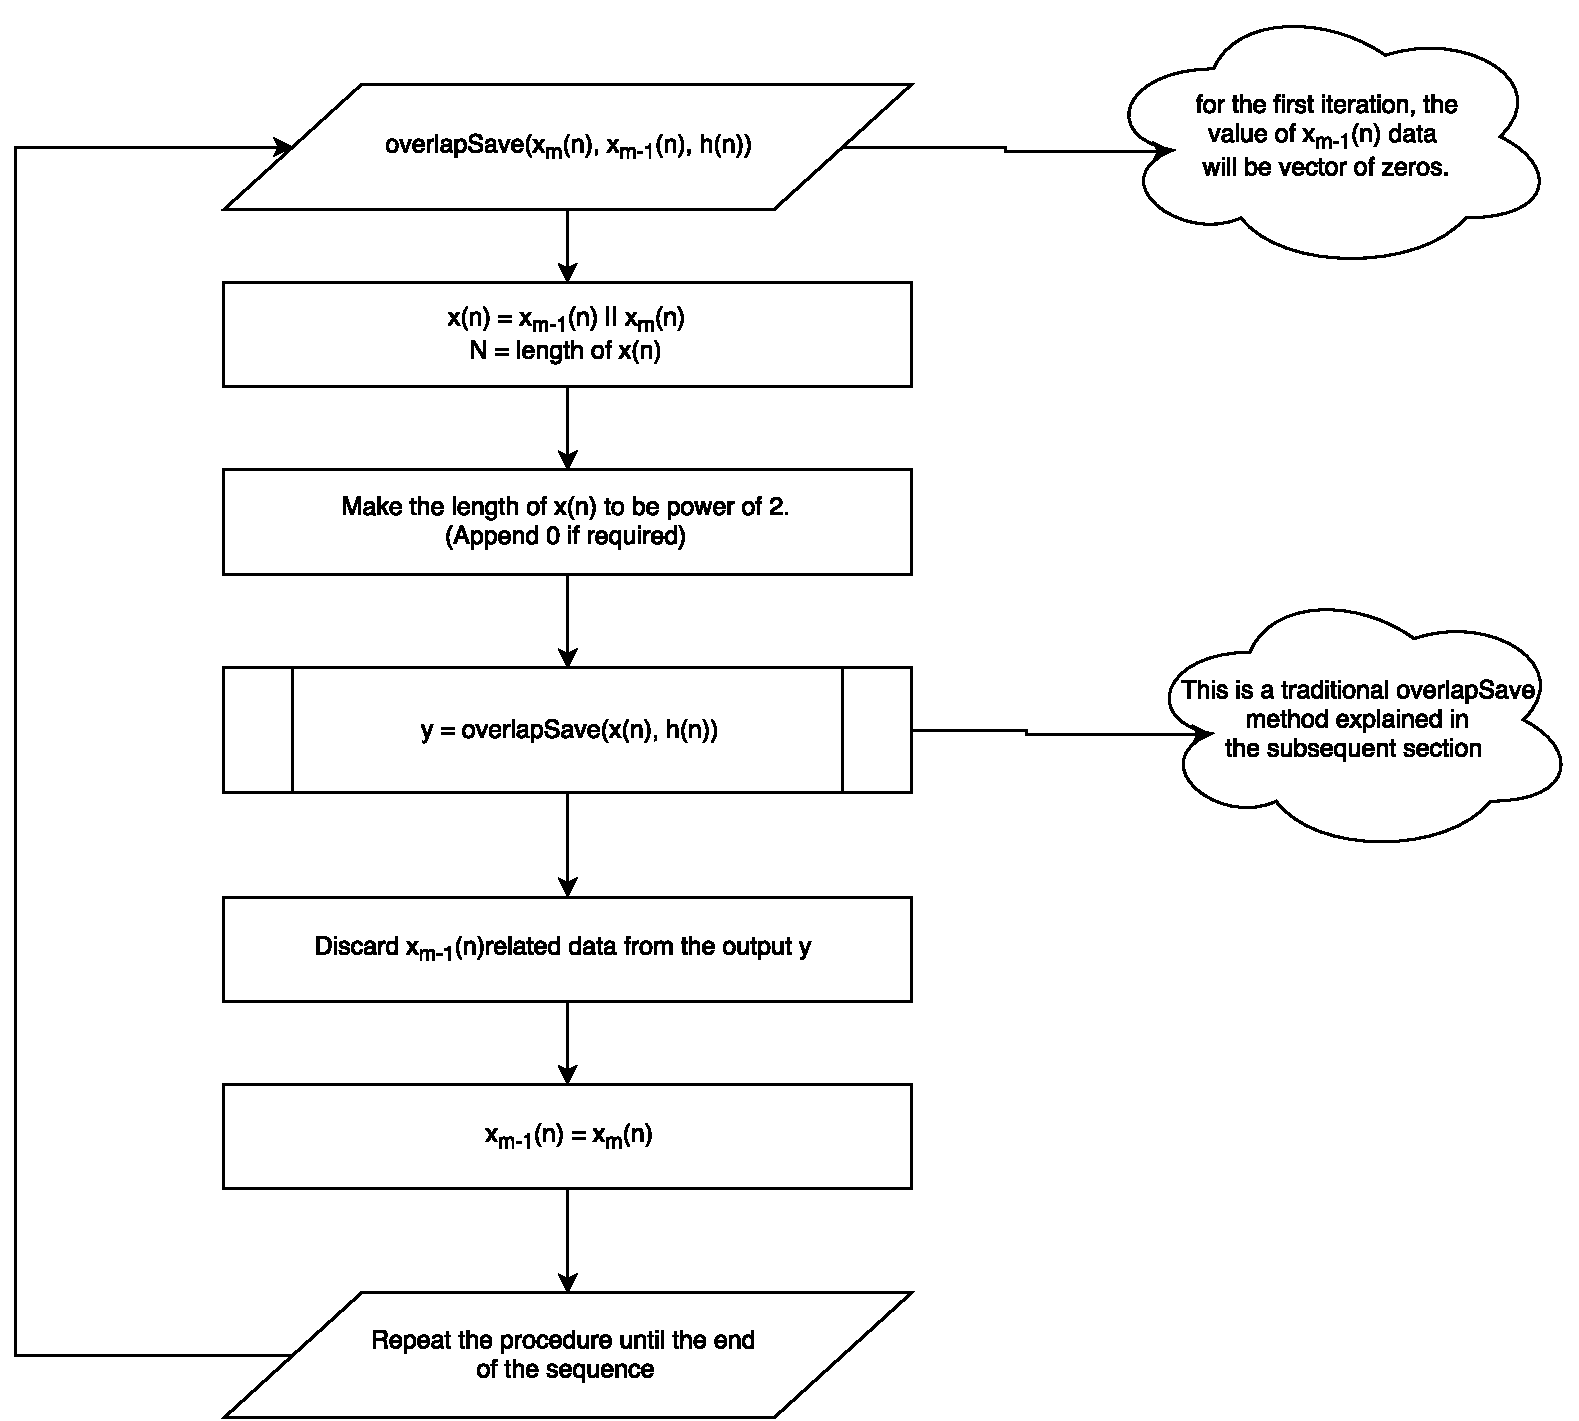
\includegraphics[width=14cm]{./algorithms/overlap_save/figures/OS_top.pdf}
	\caption{Flowchart for real-time overlap-save method}
	\label{real-time overlap-save}
	\end{figure}

\subsection*{Flowchart of traditional overlap-save method}
The following three flowcharts describe the logical flow of the traditional overlap-save method with two inputs as $overlapSave(x(n), h(n))$. In the flowchart, $x(n)$ and $h(n)$ are regarded as \textit{inTimeDomainComplex} and  \textit{inTimeDomainFilterComplex} respectively.
\subsection*{1. Decide length of FFT, data block and filter}
\begin{figure}[h]
	\centering
	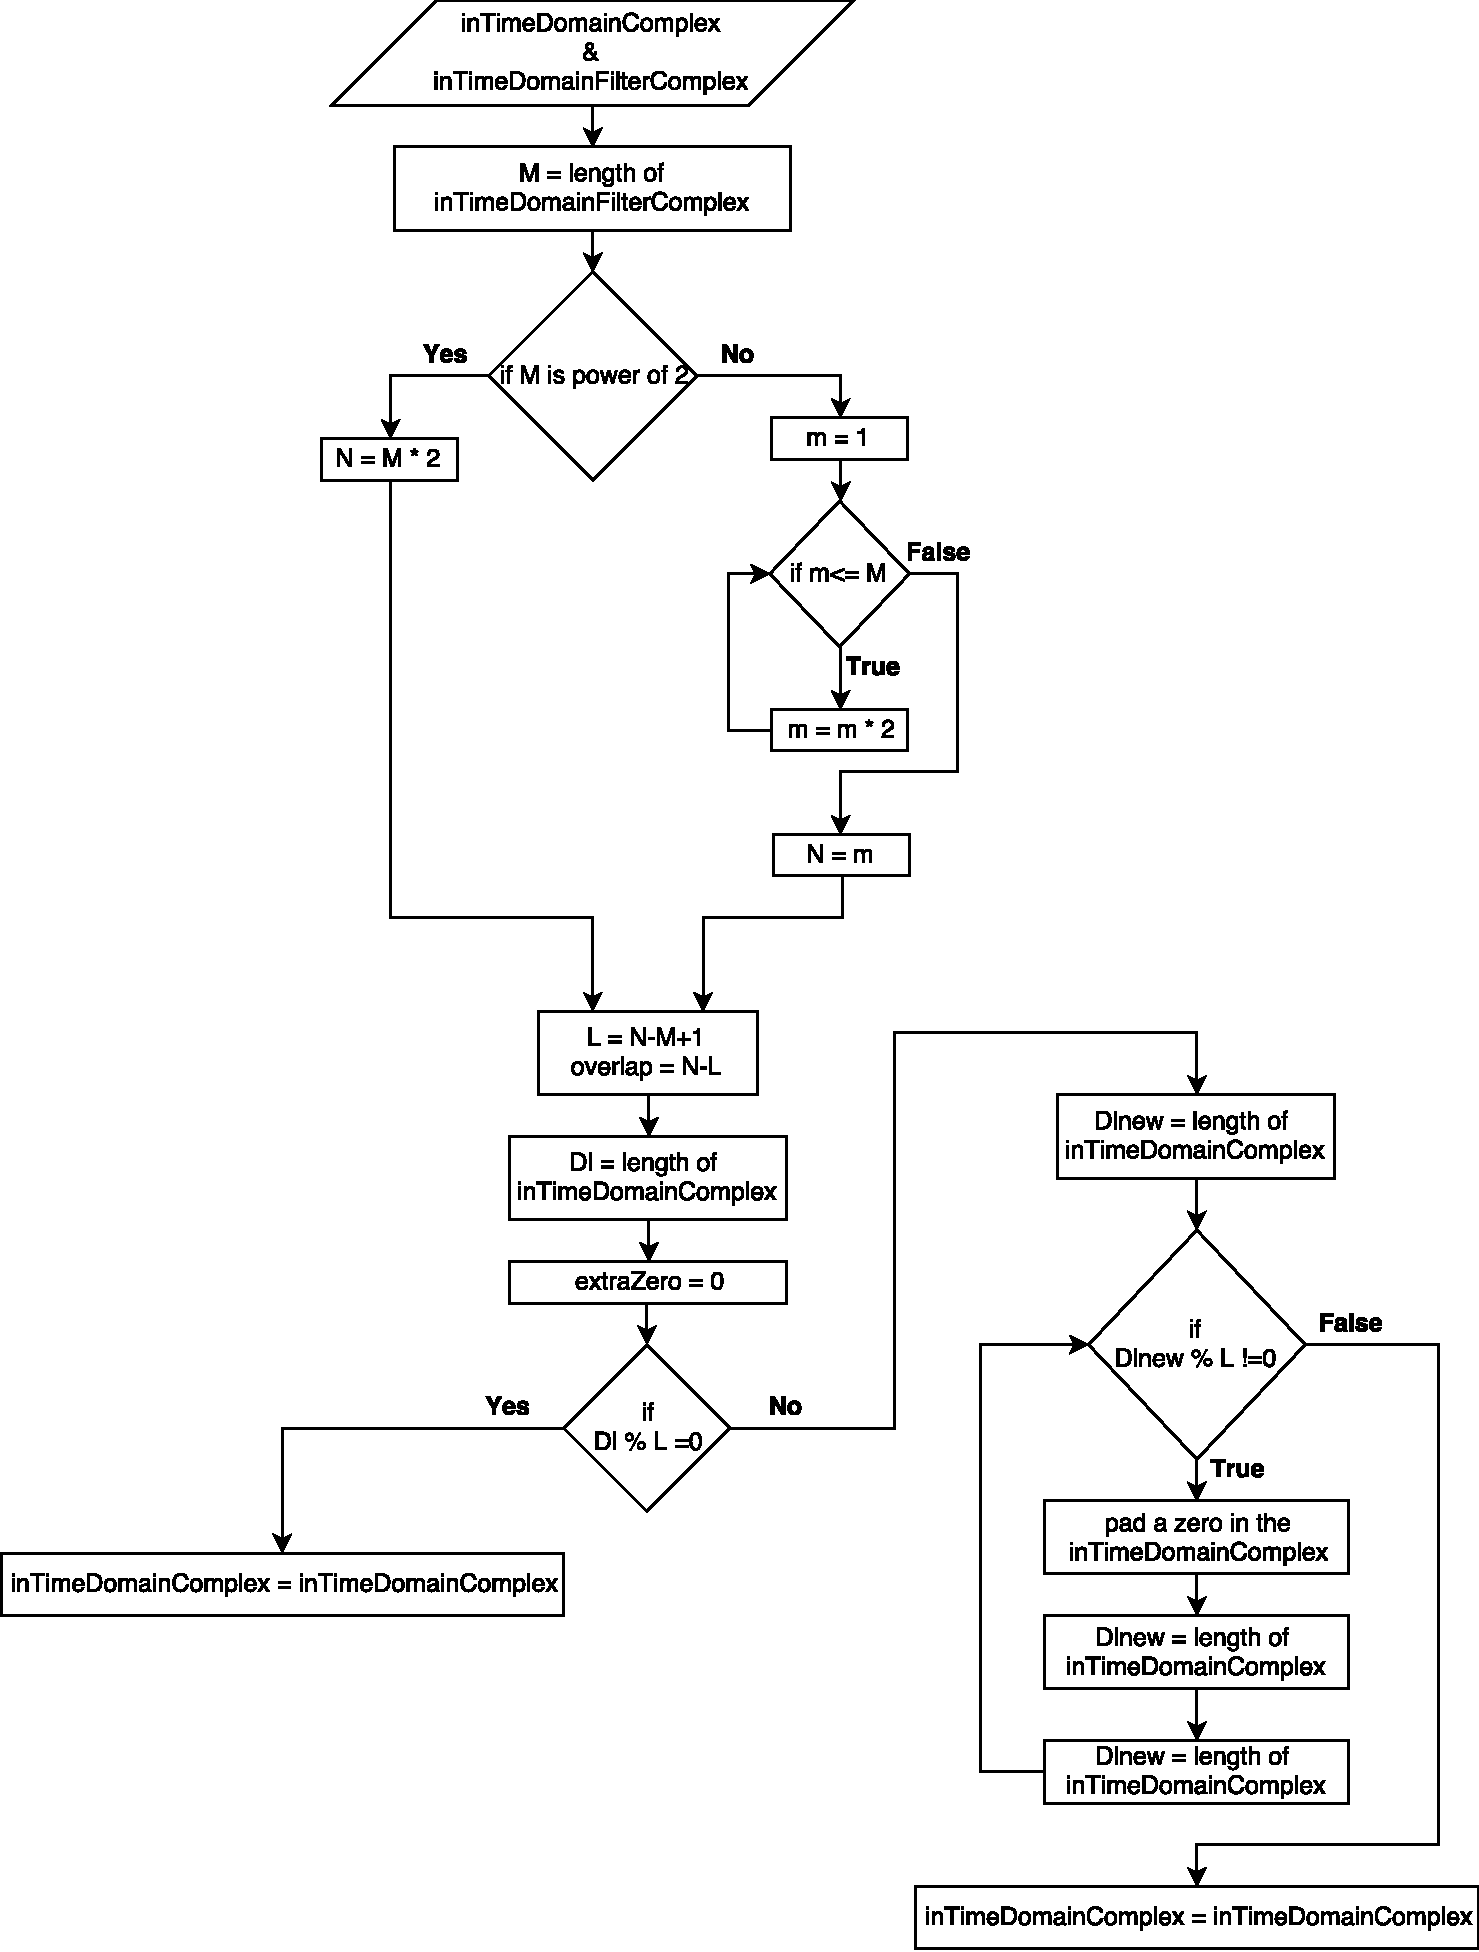
\includegraphics[width=13cm]{./algorithms/overlap_save/figures/overlapSave.pdf}
	\caption{Flowchart for calculating length of FFT, data block and filter}
	\label{overlapSave_length}
\end{figure}

\newpage
\subsection*{2. Create matrix with overlap}
\begin{figure}[h]
	\centering
	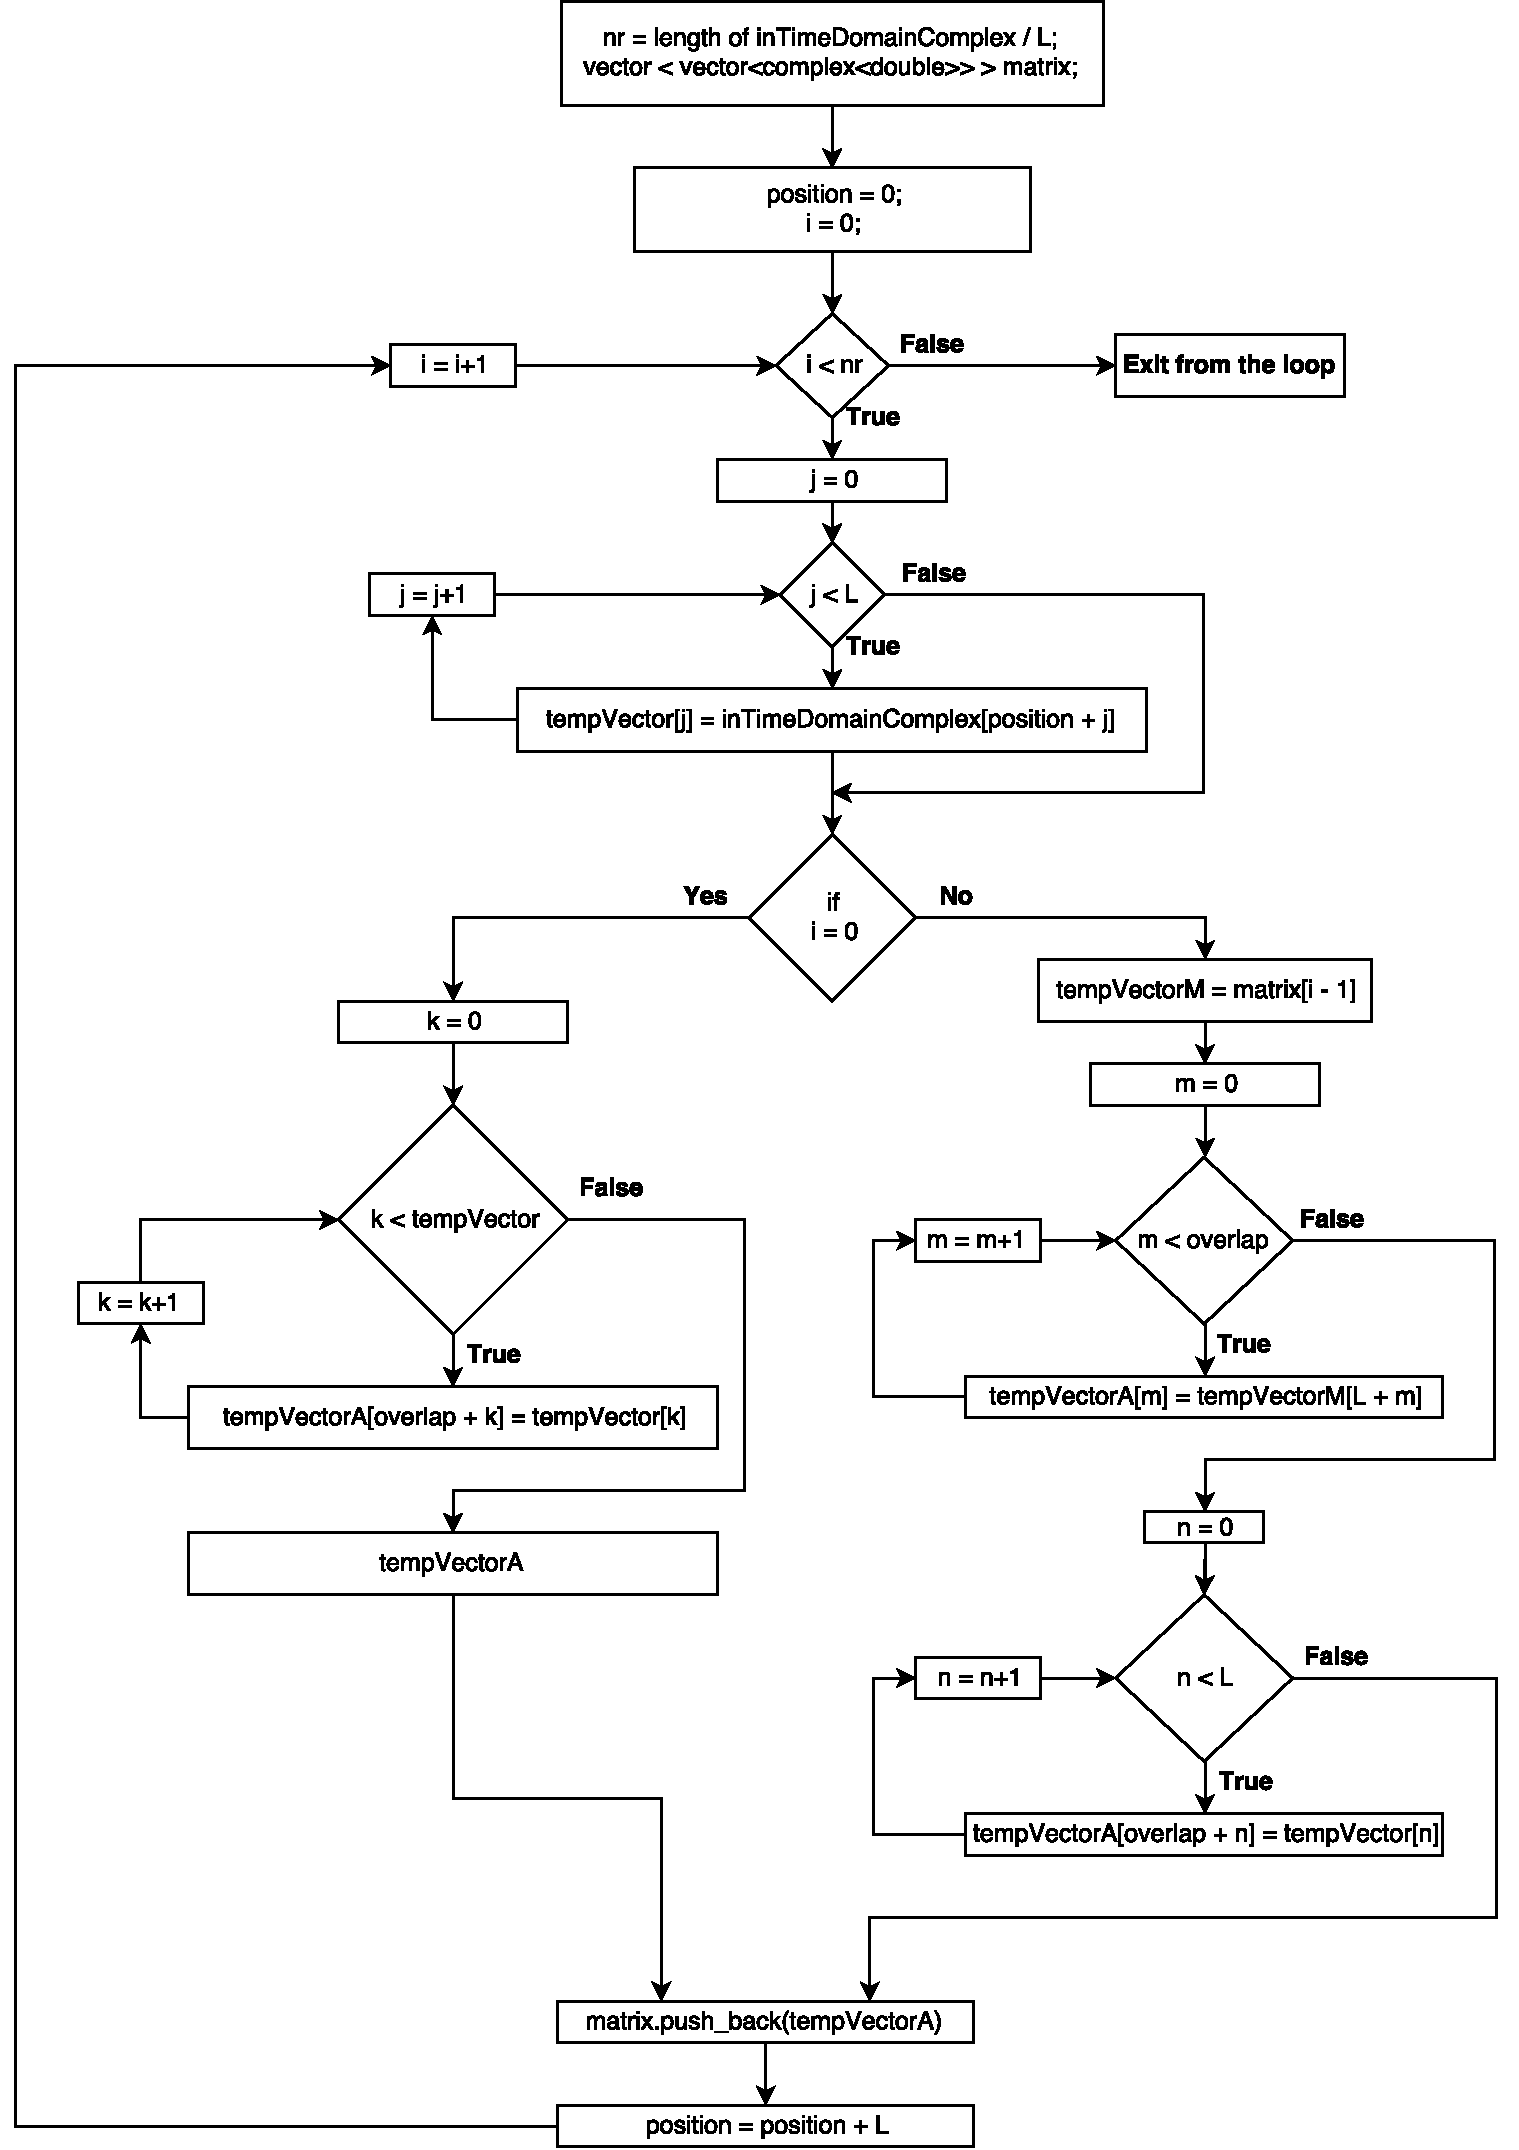
\includegraphics[width=14cm]{./algorithms/overlap_save/figures/convolution.pdf}
	\caption{Flowchart of creating matrix with overlap}
	\label{createMatrix}
\end{figure}

\newpage
\subsection*{3. Convolution between filter and data blocks}
\begin{figure}[h]
	\centering
	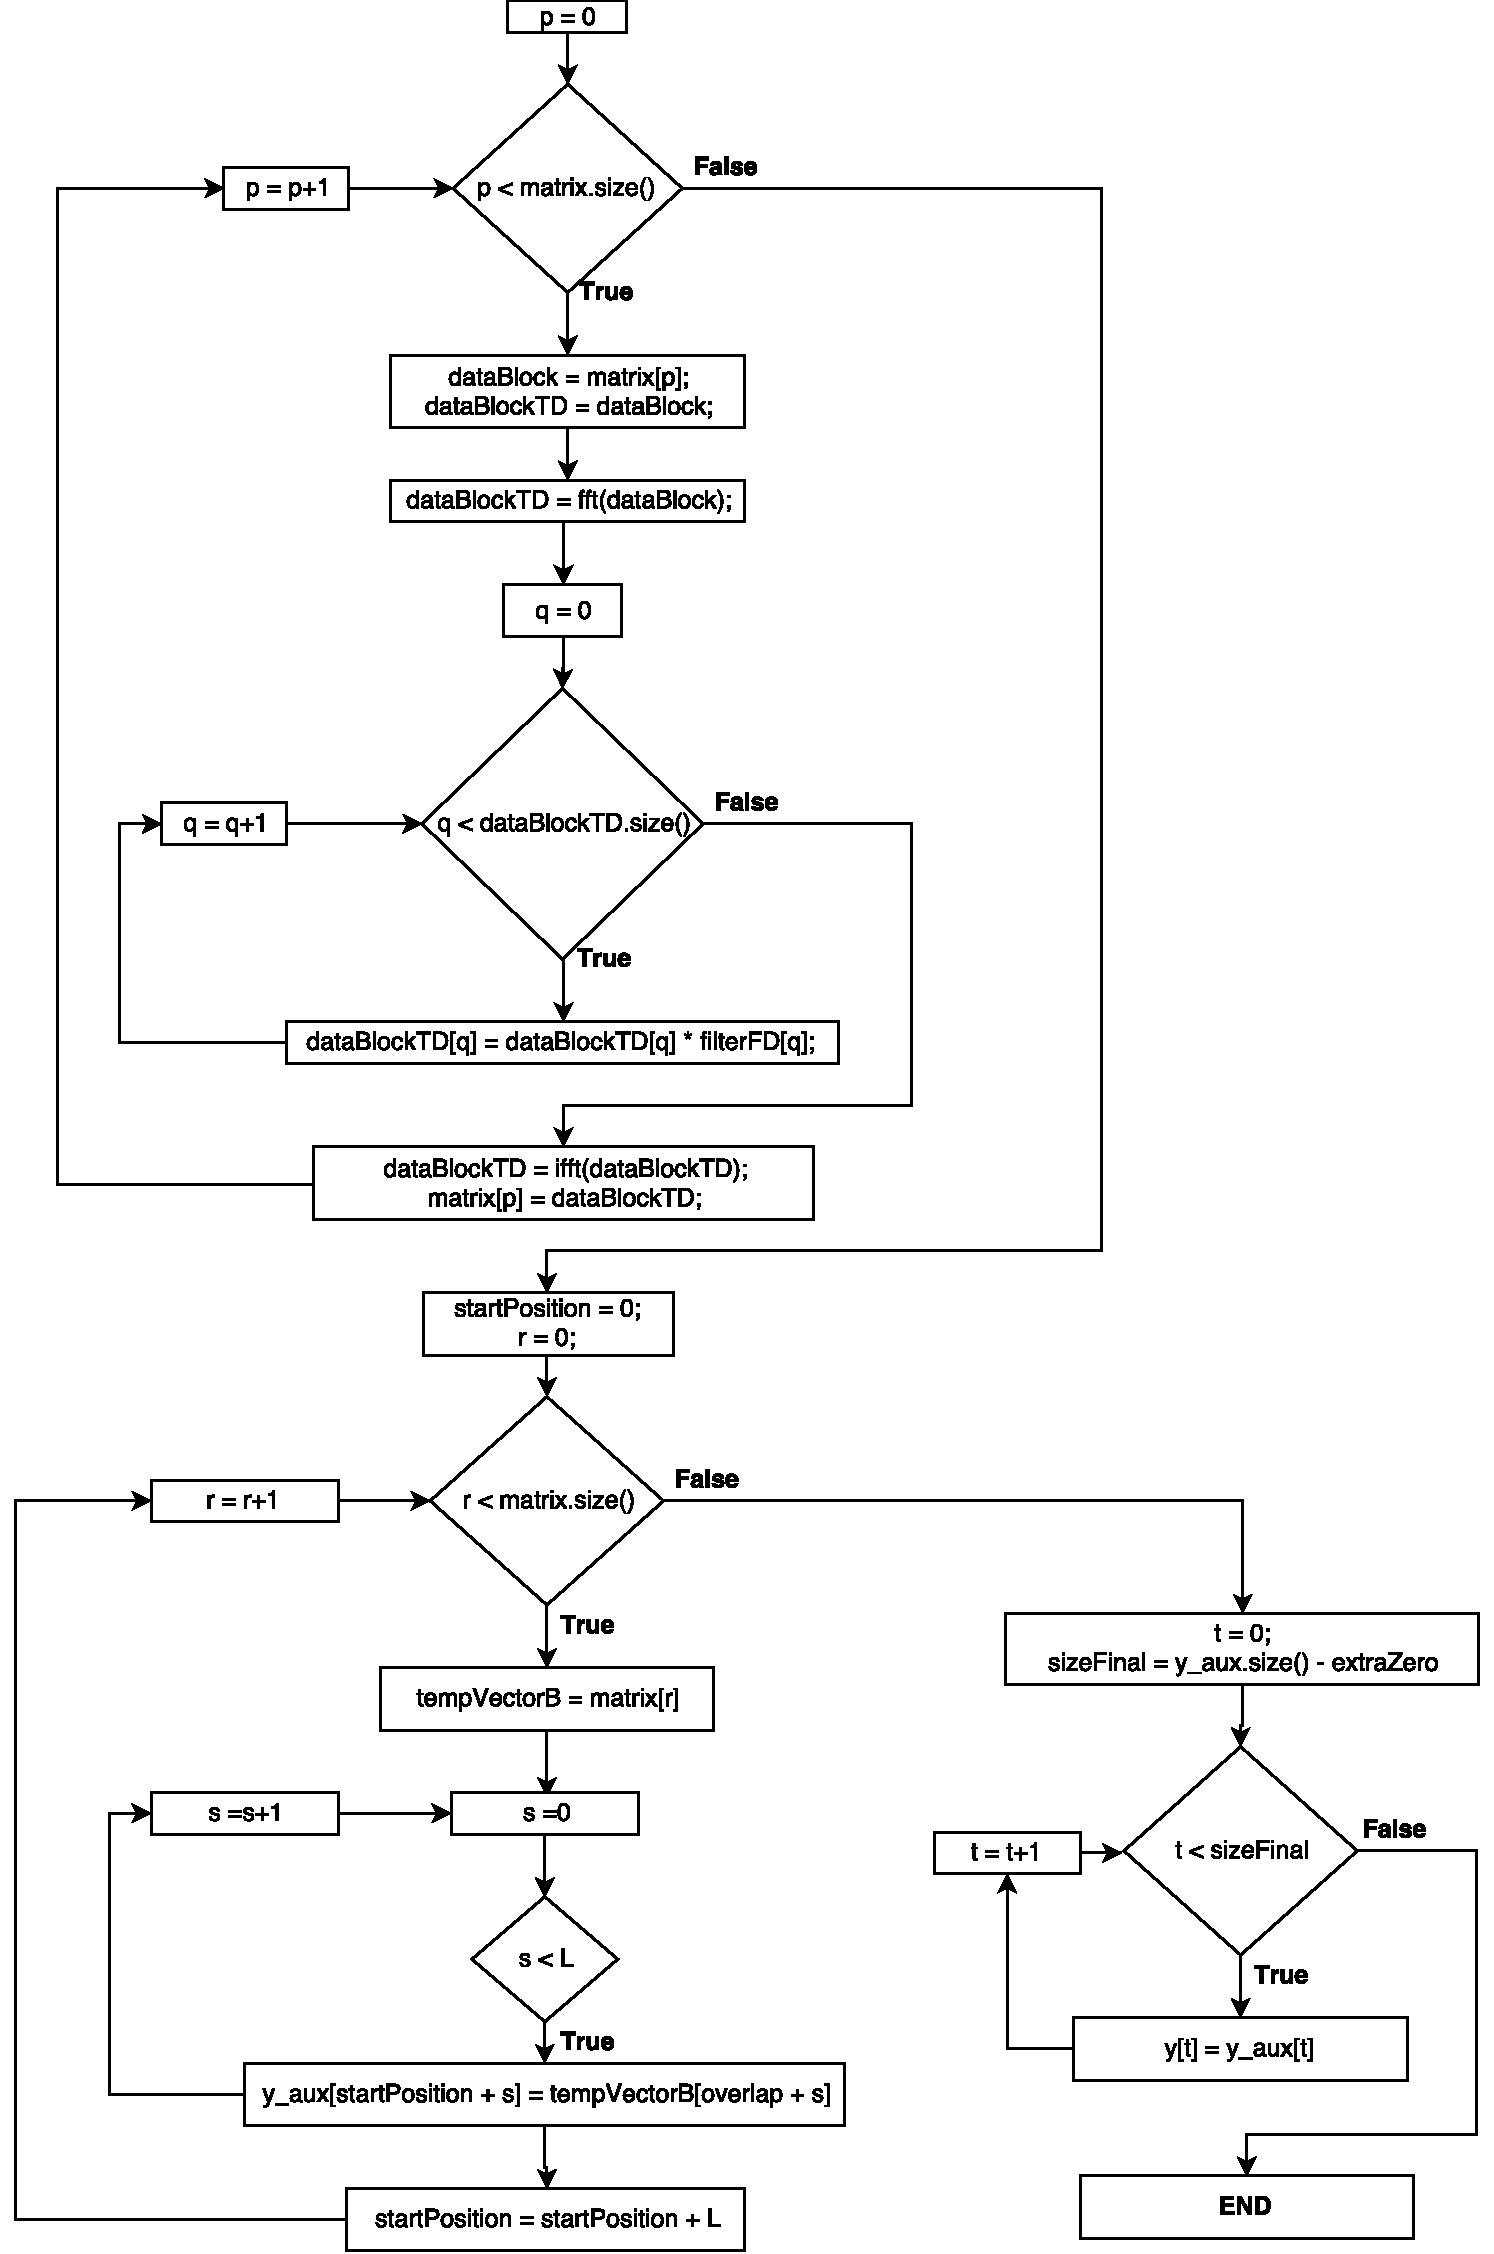
\includegraphics[width=13cm]{./algorithms/overlap_save/figures/convolution_part2.pdf}
	\caption{Flowchart of the convolution}
	\label{convolution_part2}
\end{figure}


\newpage
\subsection*{Test example of traditional overlap-save function}
This sections explains the steps of comparing our C++ based $overlapSave(x(n), h(n))$ function with the MATLAB overlap-save program and MATLAB's built-in conv() function.\\ \\
\textbf{Step 1} : Open the folder namely \textbf{overlapSave\_test} by following the path "/algorithms/overlapSave/overlapSave\_test".\\ \\
\textbf{Step 2} : Find the \textbf{overlapSave\_test.m} file and open it.\\
This overlapSave\_test.m consists of five sections:\\
\textbf{section 1 :} It generates the time domain signal and filter impulse response  and save them in the form of the text file with the name of \textit{time\_domain\_data.txt} and \textit{time\_domain\_filter.txt} respectively in the same folder.\\
\textbf{Section 2 :} It calculates the length of FFT, data blocks and filter to perform convolution using overlap-save method.\\
\textbf{Section 3 :} It consists of overlap-save code which first converts the data into the form of matrix with 50\% overlap and then performs circular convolution with filter.\\
\textbf{Section 4 :} It read \textit{overlap\_save\_data.txt} data file generated by C++ program and compare with MATLAB implementation. \\
\textbf{Section 5 :} It compares our MATLAB and C++ implementation with the built-in MATLAB function conv(). \\
\lstinputlisting[language=Matlab, caption=overlapSave\_test.m code]{../../algorithms/overlapSave/overlapSave_test/overlap_save_test.m}
\textbf{Step 3} : Choose for a sig and filt value between [1 7] and [1 3] respectively and run the first three sections namely \textbf{section 1}, \textbf{section 2} and \textbf{section 3}.\\
This will generate a \textit{time\_domain\_data.txt} and \textit{time\_domain\_filter.txt} file in the same folder which contains the time domain signal and filter data respectively.\\ \\
\textbf{Step 4} : Find the \textbf{overlapSave\_test.vcxproj} file in the same folder and open it.\\
In this project file, find \textit{overlapSave\_test.cpp} in $Source Files$ section and click on it. This file is an example of using $overlapSave$ function. Basically, \textit{overlapSave\_test.cpp} file consists of four sections:\\
\textbf{ Section 1 :} It reads the \textit{time\_domain\_data.txt} and \textit{ time\_domain\_filter.txt} files.\\
\textbf{ Section 2 :} It converts signal and filter data into complex form. \\
\textbf{ Section 3 :} It calls the $overlapSave$ function to perform convolution.\\
\textbf{ Section 4 :} It saves the result in the text file namely \textit{overlap\_save\_data.txt}.\\
\lstinputlisting[language=C++, caption=overlapSave\_test.cpp code]{../../algorithms/overlapSave/overlapSave_test/overlap_save_test.cpp}
\textbf{Step 5} : Now, go to the \textbf{overlapSave\_test.m} and run section 4 and 5.\\
It'll display the graphs of comparative analysis of the MATLAB and C++ implementation of overlapSave program and also compares results with the MATLAB conv() function.


\subsubsection{Resultant analysis of various test signals}

\subsubsection{1. Signal with two sinusoids and random noise}
\begin{figure}[h]
	\centering
	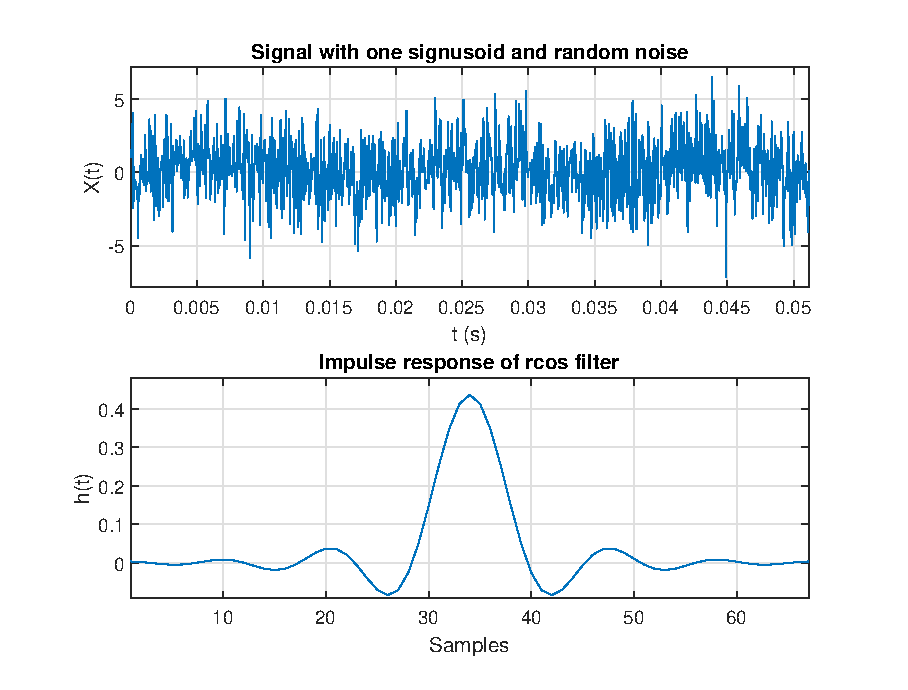
\includegraphics[width=12cm]{./algorithms/overlap_save/figures/randomNoise.eps}
	\caption{Random noise and two sinusoids signal \& Impulse response of rcos filter}\label{randomNoise}
\end{figure}

\begin{figure}[h]
	\centering
	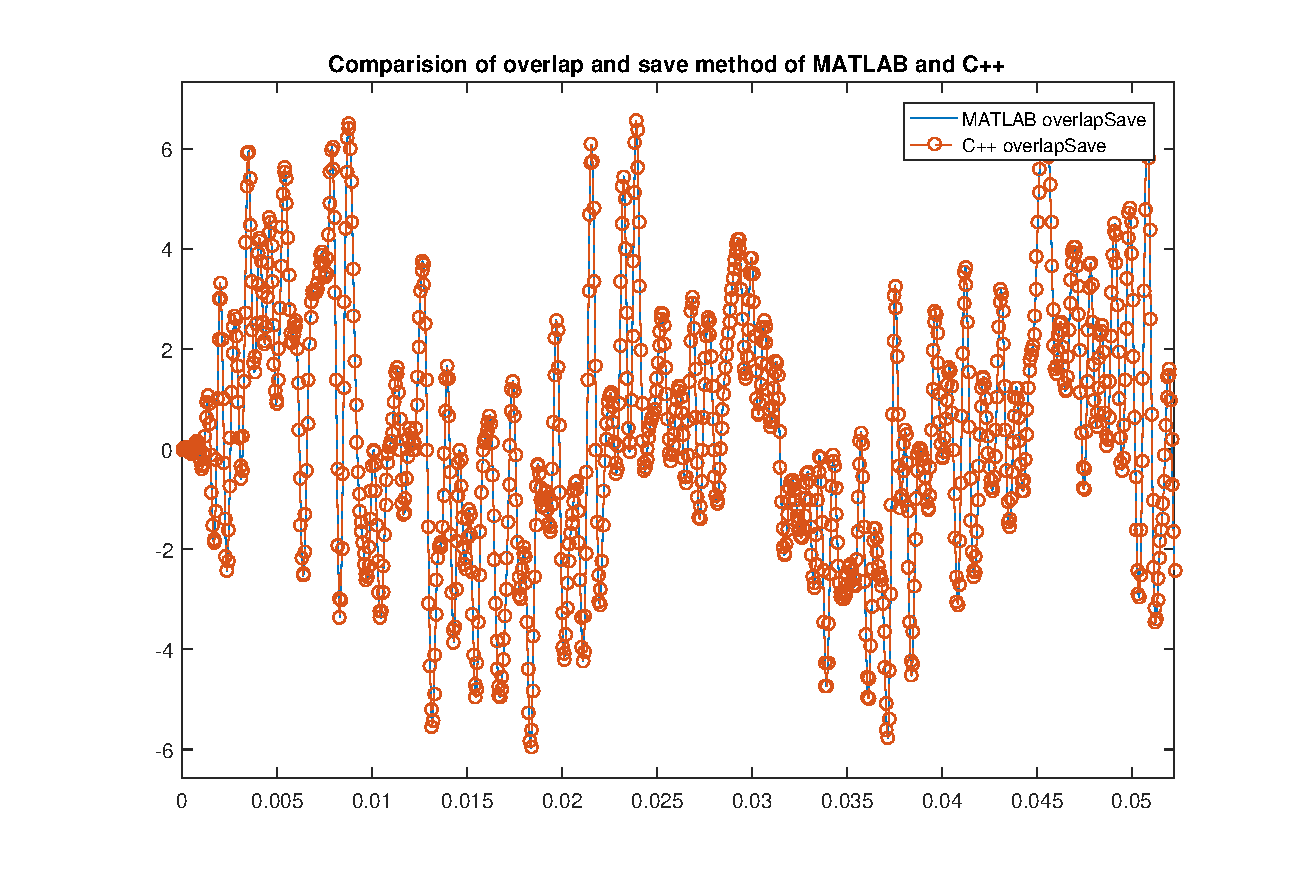
\includegraphics[width=13cm]{./algorithms/overlap_save/figures/randomNoise_matlab_and_C++.eps}
	\caption{MATLAB and C++ comparison}\label{randomNoise_matlab_and_C++}
\end{figure}

\begin{figure}[h]
	\centering
	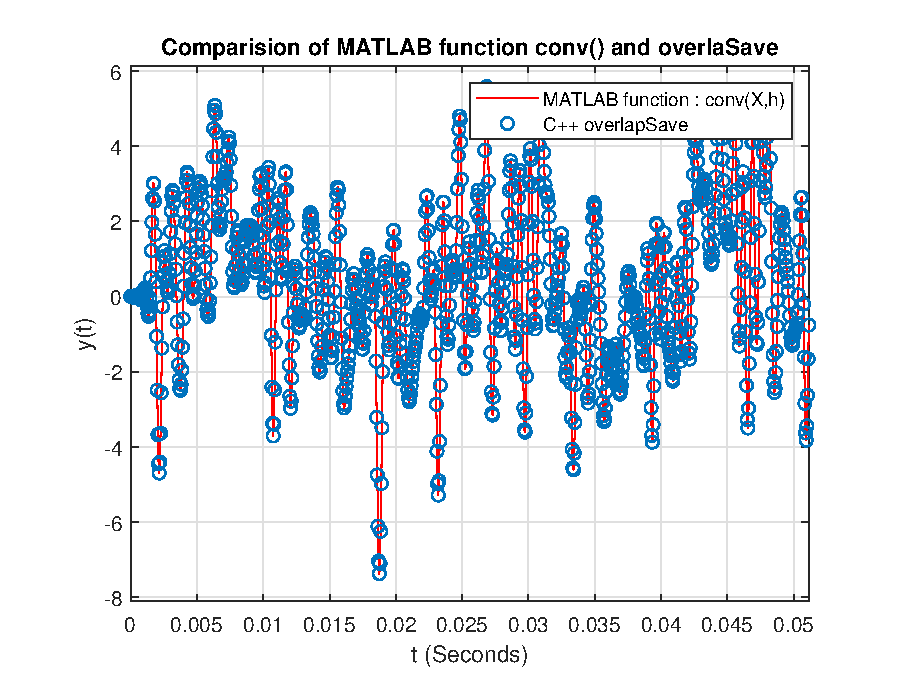
\includegraphics[width=13cm]{./algorithms/overlap_save/figures/randomNoise_conv_and_C++.eps}
	\caption{MATLAB function conv() and C++ overlapSave comparison}\label{randomNoise_conv_and_C++}
\end{figure}

\subsubsection{2. Mixed signal2}
\begin{figure}[h]
	\centering
	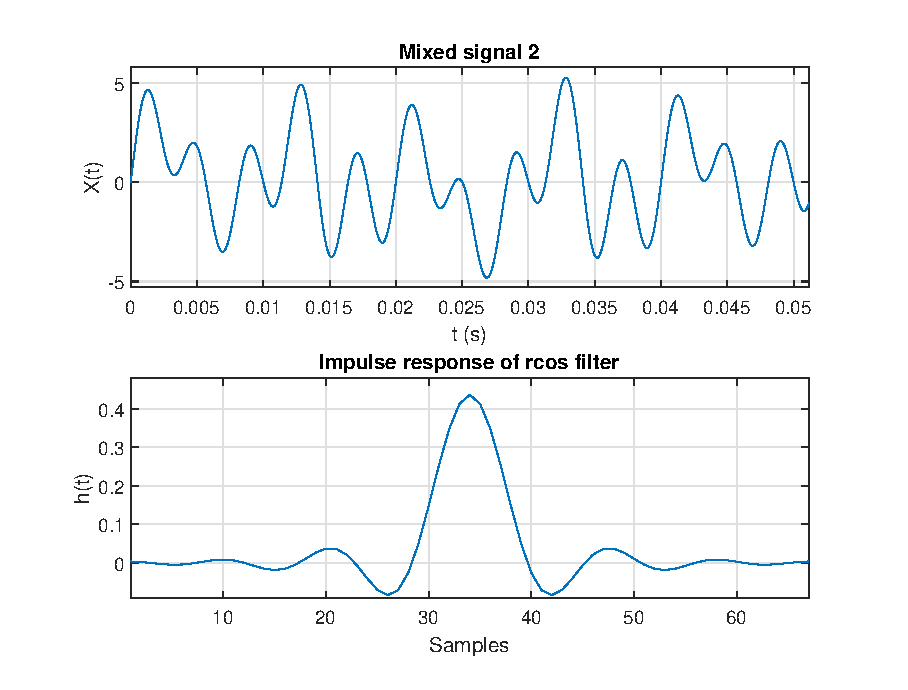
\includegraphics[width=12cm]{./algorithms/overlap_save/figures/mixed_signal2.eps}
	\caption{Mixed signal2 \& Impulse response of rcos filter}\label{mixed_signal2}
\end{figure}

\begin{figure}[h]
	\centering
	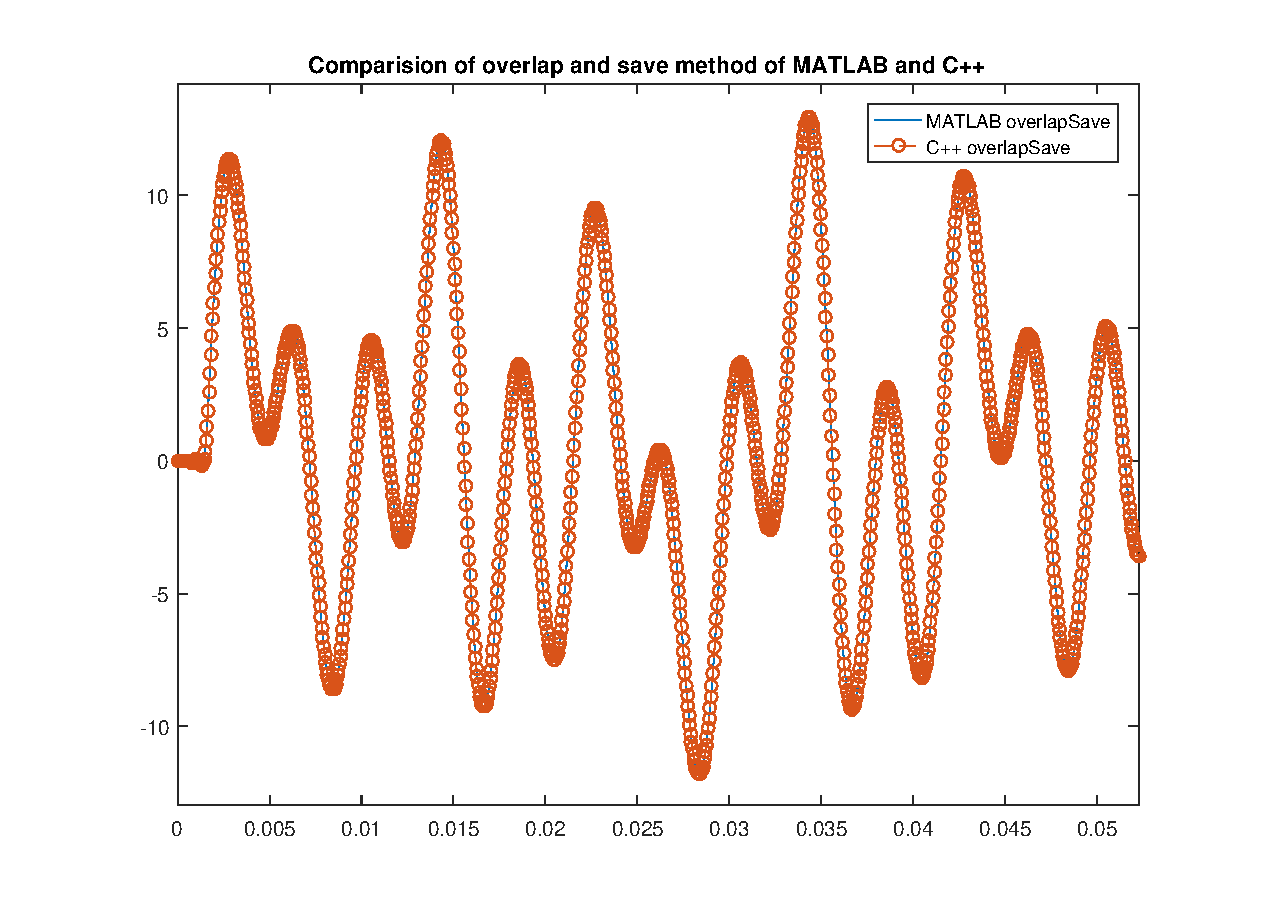
\includegraphics[width=13cm]{./algorithms/overlap_save/figures/mixed_signal2_matlab_and_C++.eps}
	\caption{MATLAB and C++ comparison}\label{mixed_signal2_matlab_and_C++}
\end{figure}

\begin{figure}[h]
	\centering
	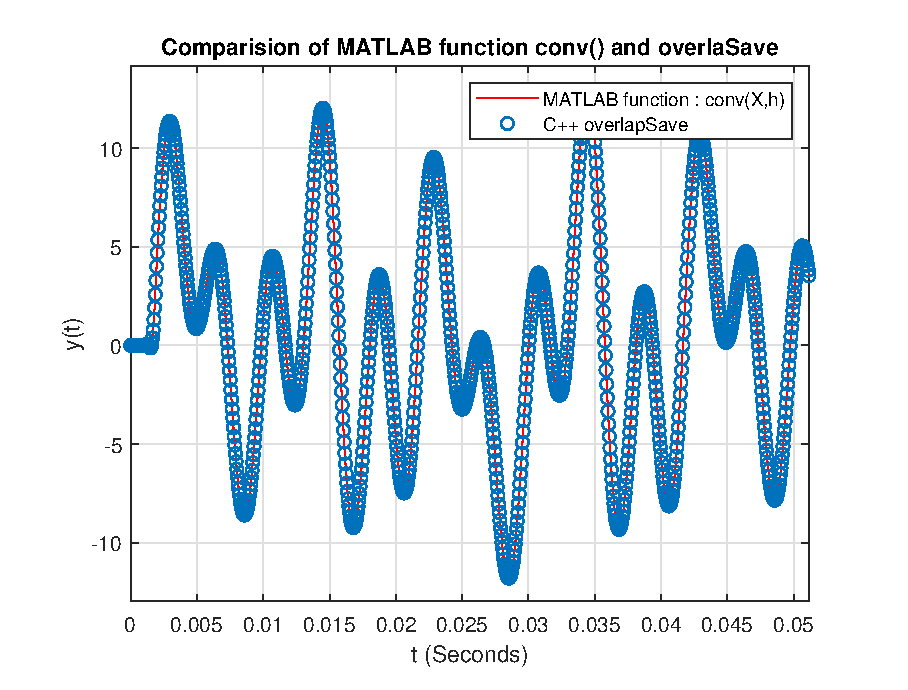
\includegraphics[width=13cm]{./algorithms/overlap_save/figures/mixed_signal2_conv_and_C++.eps}
	\caption{MATLAB function conv() and C++ overlapSave comparison}\label{mixed_signal2_conv_and_C++}
\end{figure}

\newpage

\subsubsection{3. Sinusoid with exponent}
\begin{figure}[h]
	\centering
	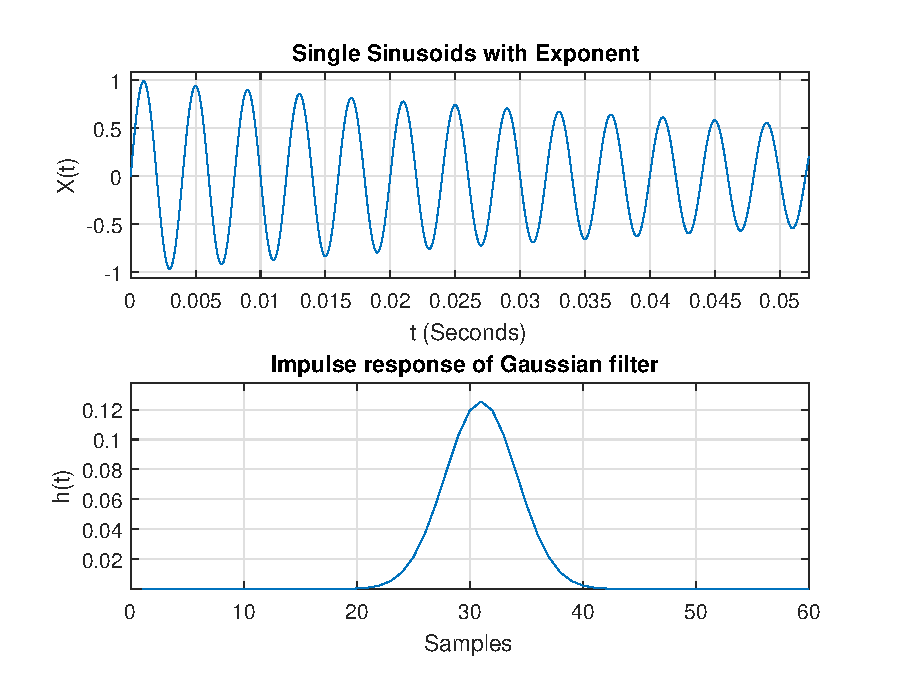
\includegraphics[width=12cm]{./algorithms/overlap_save/figures/sinusoid_with_exponent.eps}
	\caption{Sinusoid with exponent \& Impulse response of Gaussian filter}\label{sinusoid_with_exponent}
\end{figure}

\begin{figure}[h]
	\centering
	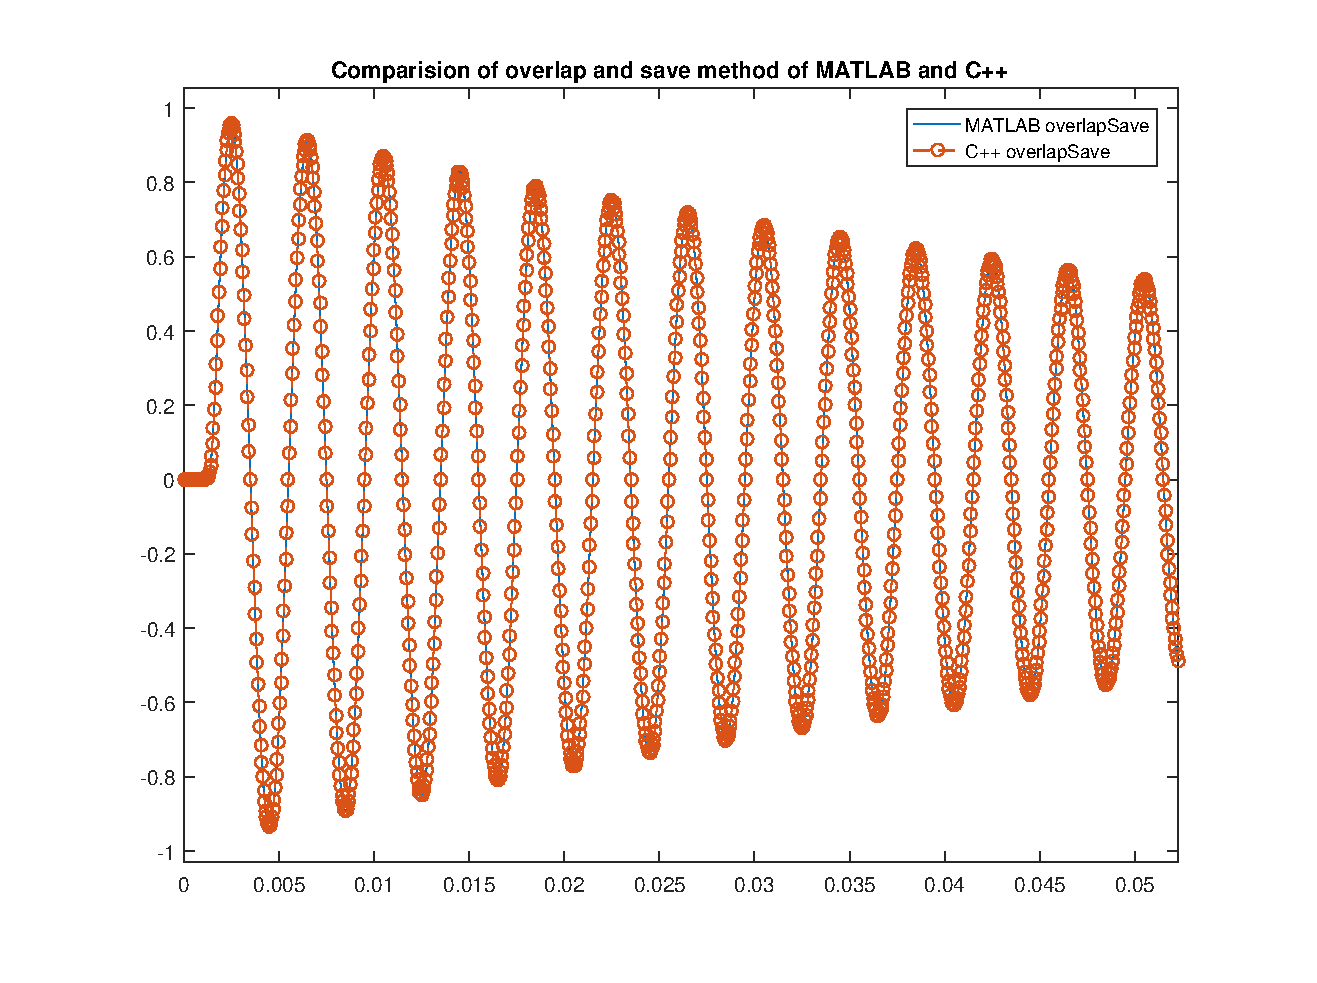
\includegraphics[width=12cm]{./algorithms/overlap_save/figures/sinusoid_with_exponent_matlab_and_C++.eps}
	\caption{MATLAB and C++ comparison}\label{sinusoid_with_exponent_matlab_and_C++}
\end{figure}

\begin{figure}[h]
	\centering
	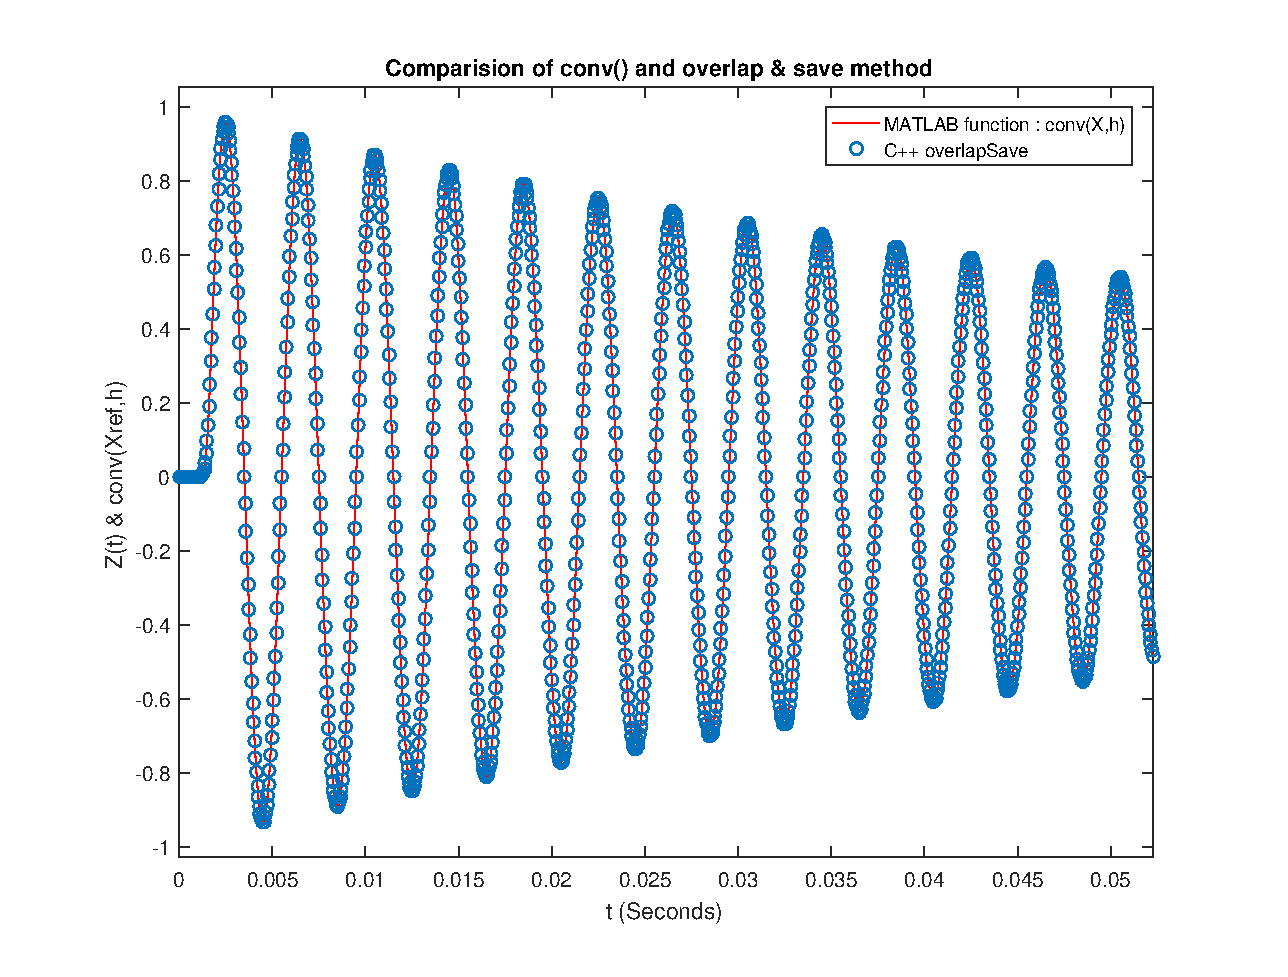
\includegraphics[width=11cm]{./algorithms/overlap_save/figures/sinusoid_with_exponent_conv_and_C++.eps}
	\caption{MATLAB function conv() and C++ overlapSave comparison}\label{sinusoid_with_exponent_conv_and_C++}
\end{figure}

\newpage
\subsection*{Test example of real-time overlap-save function with Netxpto simulator}
% $overlapSave(x_{m-1}(n), x_{m}(n), h(n))$ 
This section explains the steps of comparing real-time overlap-save method with the time-domain filtering. The structure of the real-time overlap-save function $overlapSave(x_{m-1}(n), x_{m}(n), h(n))$ requires an impulse response $h(n)$ of the filter. There are two methods to feed the impulse response to the real-time overlap-save function:\\
\textbf{Method 1.} The impulse response $h(n)$ of the filter can be fed using the time-domain impulse response formula of the filter.\\
\textbf{Method 2.} Write the transfer function of the filter and convert it into the impulse response using Fourier transform method. \\
Here, this example uses the method 2 to feed the impulse response of the filter. In order to compare the result, follow the steps given below:\\ \\
\textbf{Step 1} : Open the folder namely \textbf{overlapSaveRealTime\_test} by following the path "/algorithms/overlapSave/overlapSaveRealTime\_test".\\ \\
\textbf{Step 2} : Find the \textbf{overlapSaveRealTime\_test.vcxproj} file and open it.\\
In this project file, find \textit{filter\_20180306.cpp} in $Source Files$ section and click on it. This file includes the several definitions of the two different filter class namely \textbf{FIR\_Filter} and \textbf{FD\_Filter} for filtering in time-domain and frequency-domain respectively. In this file, \textbf{FD\_Filter::runBlock} displays the logic of real-time overlap-save method.\\
\lstinputlisting[firstline=1, lastline=150, language=C++, caption=filter\_20180306.cpp code]{../../algorithms/filter/filter_20180306.cpp}
\textbf{Step 3} : Next, open \textbf{overlapSaveRealTime\_test.cpp} file in the same project and run it. Graphically, this files represents the following Figure \ref*{realTimeOverlapSave}.\\
\begin{figure}[h]
	\centering
	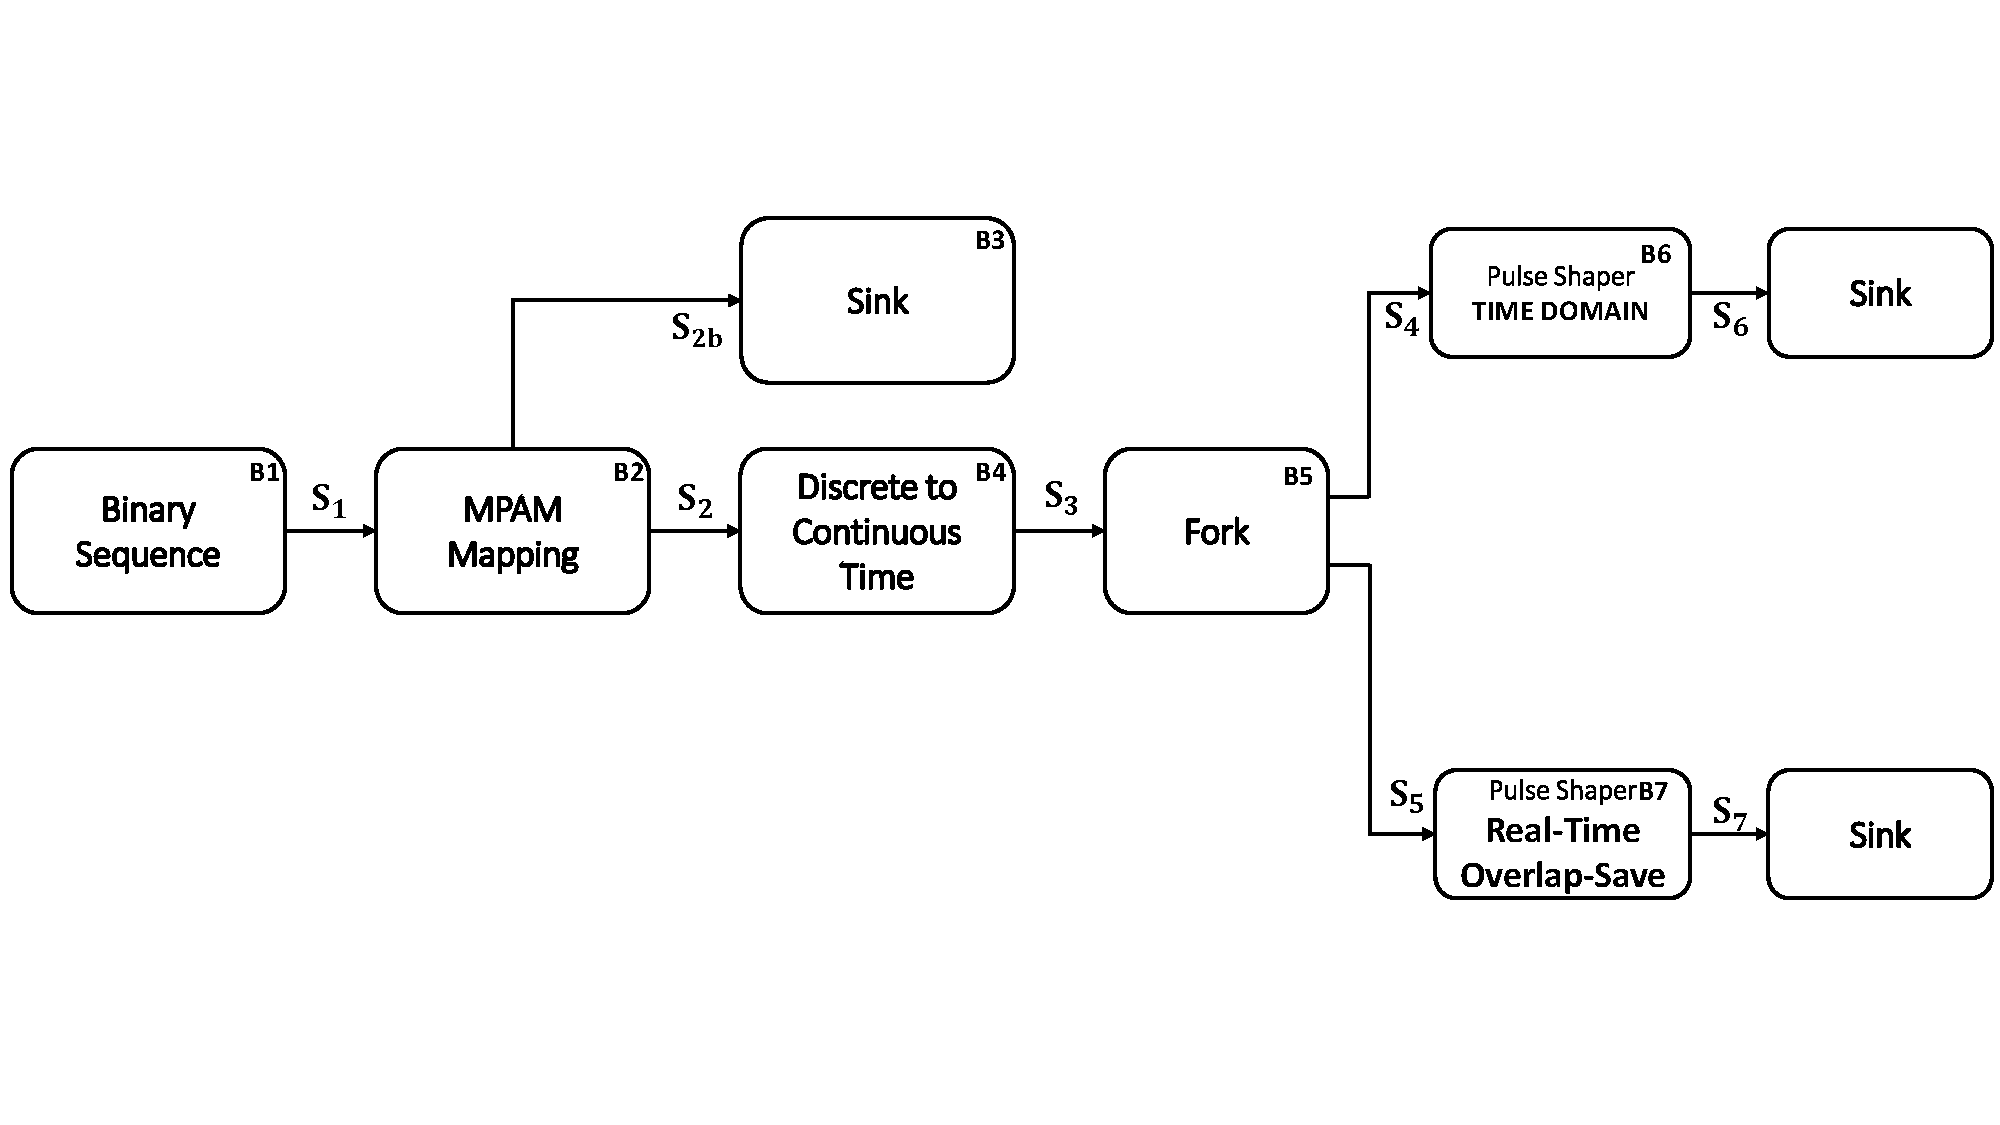
\includegraphics[width=12cm]{./algorithms/overlap_save/figures/realTimeOverlapSave.pdf}
	\caption{Real-time overlap-save example setup}\label{realTimeOverlapSave}
\end{figure}\\
\textbf{Step 4} : Open the MATLAB visualizer and compare the signal \textbf{S6.sgn} and \textbf{S7.sgn} as shown in Figure \ref{S6S7}.
\begin{figure}[h]
	\centering
	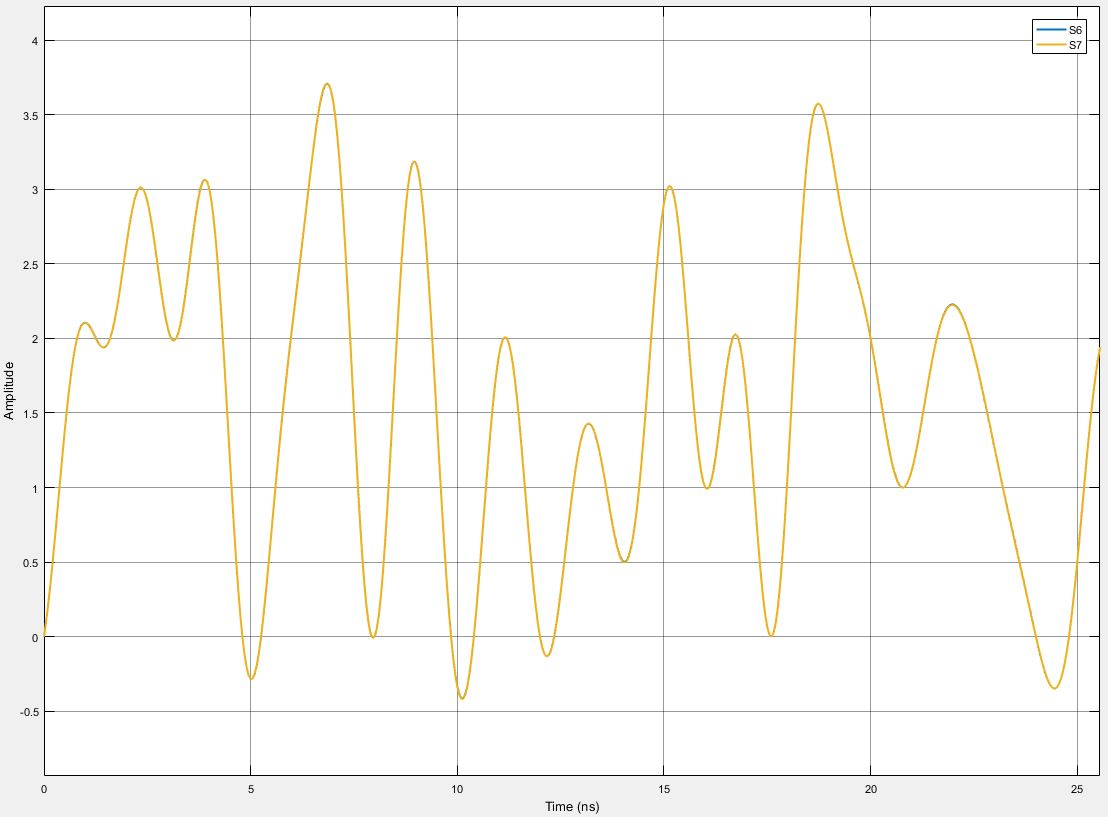
\includegraphics[width=12cm]{./algorithms/overlap_save/figures/S6_S7.jpg}
	\caption{Comparison of signal S6 and S7}\label{S6S7}
\end{figure}

\begin{thebibliography}{1}
 \bibitem{notes} Blahut, R.E. {\em Fast Algorithms for Digital Signal Processing}, Addison-Wesley, Reading, MA,
 1985.
 \bibitem{notes} Steven W. Smith. {\em The Scientist and Engineer's Guide to Digital Signal Processing.} California Technical Publishing, San Diego, CA, USA, 1997.
\end{thebibliography}

%\end{document}

